\documentclass[11pt]{article} % use larger type; default would be 10pt
\usepackage[utf8]{inputenc} % set input encoding (not needed with XeLaTeX)
\usepackage{fullpage}
\usepackage{graphicx} % support the \includegraphics command and options
\usepackage{caption}
\usepackage{subcaption}
\usepackage{amsmath}
\usepackage{amssymb}
\usepackage{lscape}
\usepackage{pdflscape}
\usepackage{float}
\usepackage{titlesec}
\usepackage{physics} %TODO convert everything else across to this
\newcommand{\drv}[2]{\ensuremath{\frac{d #1}{d #2}}}
\newcommand{\ddrv}[2]{\ensuremath{\frac{d^2 #1}{d^2 #2}}}
\newcommand{\into}{\ensuremath{\int_{-1}^1}}
\newcommand{\intz}{\ensuremath{\int_0^1}}
\newcommand{\intf}{\ensuremath{\int_{-\infty}^\infty}}
\newcommand{\inti}{\ensuremath{\int_{x_{i-1/2}}^{x_{i+1/2}}}}
\newcommand{\intO}{\ensuremath{\int_{4\pi}}}
%\newcommand{\order}[1]{\ensuremath{\mathcal{O}(#1)}}
\newcommand{\He}{\ensuremath{\mbox{He}}}
\newcommand{\expv}[1]{\ensuremath{\mathbb{E}[ #1]}}
\newcommand{\xs}[2]{\ensuremath{\Sigma_{#1}^{(#2)}}}


\title{Tests for UQ Framework}
\author{Paul Talbot}
%\date{}

\begin{document}
\maketitle
\section{Introduction}
This work outlines the development of an uncertainty quantification (UQ) framework using generalized polynomial chaos expansions and stochastic collocation (PCESC), verified using Monte Carlo (MC) sampling.  The intended use is as a ``black-box wrapper,'' agnostic of the algorithm whose uncertaintly is quantified.  To verify the several stages this framework undergoes in development and its independence from any deterministic solver, we present here several test codes of increasing complexity that the UQ framework will act on.  The four test codes solve four problems: a polynomial expression; 1D mono-energetic neutron transport in a semi-infinite medium with uniform source and single material; 1D $k$-eigenvalue neutron diffusion transport with two energy groups and a single material; and a 2D, two energy group $k$-eigenvalue neutron diffusion transport quarter-core benchmark.

\subsection{Algorithm}
Each problem-solving code is treated as a black box that reads in an input file and produces a result readable from an output file.  The problem-solving code can be represented as a function $U$ of certain input parameters $\theta$ in deterministic parameter space $\Theta$ and uncertain parameters $Y(\omega)$ in uncertainty space $\Gamma$, where $Y$ could be a single parameter or a vector of uncertain parameters and $\omega$ is a single realization in the uncertainty space $\Gamma$.  We expand $U(\theta,Y)$ in basis polynomials characteristic of the uncertain parameters:
\begin{equation}
U(\theta;Y)\approx U_P(\theta;Y) \equiv \sum_{p=0}^P u_p(\theta) \psi_p(Y),
\end{equation}
Generally, we omit the dependency $\theta$ when considering stochastic space ($U(\theta;Y)=U(\theta))$.
$u_p(\theta)$ are polynomial expansion coefficients, $\psi_p(Y)$ are orthonormal basis polynomials, and the sum is necessarily truncated at finite order $P$.  In the limit as $P$ approaches infinity (or if $U(Y)$ can be expressed exactly as a polynomial of order $P$), there is no approximation.  Ideally the expansion converges after a reasonably small number of terms.

We make use of the orthonormal nature of the polynomial basis to calculate the coefficients $c_i$,
\begin{equation}
u_p(\theta) = \int_\Gamma U(Y)\psi_p(Y)dY.
\end{equation}
With the right choice of polynomials, we can apply quadrature to solve the integral,
\begin{equation}
u_p = \sum_{\ell=0}^{L} w_\ell U(Y_\ell) \psi_p(Y_\ell).
\end{equation}
In this case we are applying Gaussian quadrature, where an expansion of order $L$ can exactly integrate a polynomial of order $2L-1$.  While the order of the polynomial $\psi_p(Y_\ell)$ is $p$, the equivalent polynomial order of $U(Y_\ell)$ is unknown and must be determined or approximated.  If $U(Y)$ is scalar, $L$ need only be $(p+1)/2$; this is the low bound for quadrature order.  Coefficient convergence as a function of quadrature order is further explored for some of the cases in this report (see \S \ref{sec:quadconv}).

Once the coefficients are calculated, they in combination with the basis polynomials create a reduced-order model that can be sampled like the original function, but ideally at much less computational expense.  The measure of success for the PCESC algorithm is its ability to preserve the mean and variance of the original function, as well as produce a virtually identical probability density function (pdf) for the solution quantity of interest, $U(\theta;Y)$.  The mean, variance, and pdf are confirmed using brute-force Monte Carlo sampling of the original code.

\section{Solvers}
In this section we identify the four deterministic solvers on which uncertainty propagation will be applied.

\subsection{}

\section{Univariate UQ}
In this section we limit ourselves to the analysis of the UQ algorithm as it applies to univariate versions of the deterministic solvers.  This gives a baseline before approaching multivariate inputs in their variety.

\subsection{Polynomial Solver: $f(x)$}
The purpose of the polynomial solver is to demonstrate convergence on an analytic mean, variance, and pdf for both Monte Carlo and PCESC methods.  We consider two cases.  In the first, $x$ is distributed uniformly as $x\sim\mathcal{U}(3,7)$.  In the second, $x$ is distributed normally as $x\sim\mathcal{N}(5,4)$.  The expected analytic moments are given in Table \ref{tab:poly uni mom}.
\begin{table}[H]
\centering
\begin{tabular}{c|c|c}
Distribution & $m_1$ & var \\ \hline
$\mathcal{U}(3,7)$ & 11 & 79/3\\
$\mathcal{N}(5,4)$ & 11 & 16
\end{tabular}
\caption{Analytic Moments for Univariate Polynomial Solver}
\label{tab:poly uni mom}
\end{table}
Because this case expands a first-order polynomial in polynomials, it can be exactly replicated with a first-order expansion.  Table \ref{tab:poly uni res} shows the Monte Carlo and PCESC statistics.  The solution PDFs are in Fig. \ref{fig:poly uni res}.

\begin{table}[H]
\begin{center}
\begin{tabular}{c|c c|l l}
Distr. & UQ & runs$|$order & mean & variance \\ \hline
Uniform & MC & $1\times10^7$ & 10.999555712 & 5.3374535046 \\
 & SC & 2 & 11.0 & 5.33333333333 \\ \hline
Normal & MC & $1\times10^7$ & 11.0000448162 & 15.9892244775 \\
 & SC & 2 & 11 & 16 
\end{tabular}
\end{center}
\caption{Polynomial Solver, Univariate Statistics}
\label{tab:poly uni res}
\end{table}

\begin{figure}[H]
\centering
  \begin{subfigure}[b]{0.4\textwidth}
   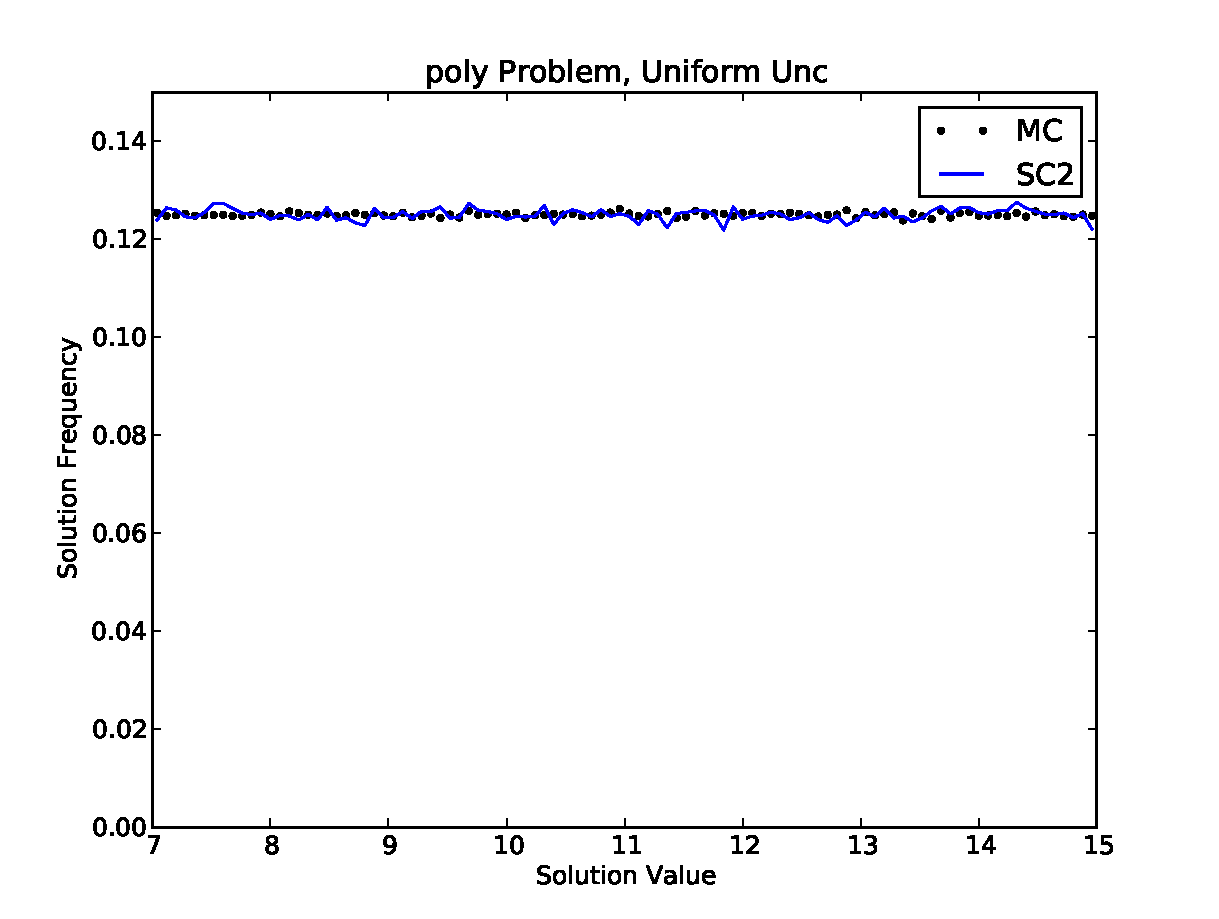
\includegraphics[width=\textwidth]{../graphics/poly_uniform_pdfs}
   \caption{Uniform}
      \label{fig:poly uni}
  \end{subfigure}
  \begin{subfigure}[b]{0.4\textwidth}
   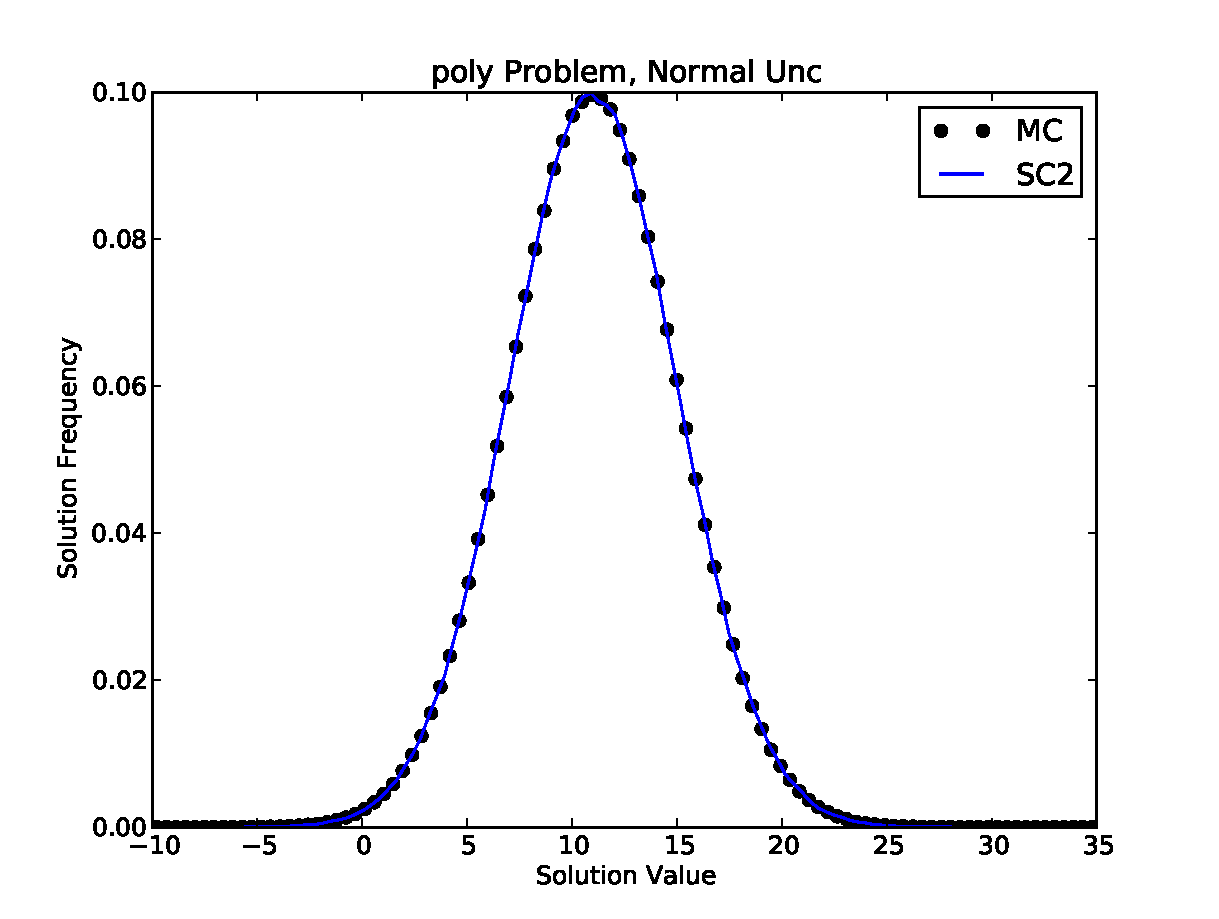
\includegraphics[width=\textwidth]{../graphics/poly_normal_pdfs}
   \caption{Normal}
      \label{fig:poly norm}
  \end{subfigure}
  \caption{Univariate Polynomial Solver PDFs}
  \label{fig:poly uni res}
\end{figure}

\subsection{Source Solver: $\phi=\phi\qty(S,D,x,\Sigma_a)$}
For the univariate case, we introduce uncertainty in the absorption cross section $\Sigma_a$.  We consider two cases: first, when $\Sigma_a\sim\mathcal{U}(0.5,1)$; second, when $\Sigma_a\sim\mathcal{N}(0.75,0.0225)$.  The other parameters are
\begin{align}
S &= 1.0 \text{ n/cm}^2\text{/s},\\
D &= 0.5 \text{ /cm},\\
x &= 2.0 \text{ cm}.
\end{align}
We consider several increasing levels of polynomial expansion and the convergence onto the Monte Carlo solution.  The results are in Table \ref{tab: source uni res}.  The solution PDFs are in Fig. \ref{fig:source uni res}.

\begin{table}[H]
\begin{center}
\begin{tabular}{c|c c|l l}
Distr. & UQ & runs$|$order & mean & variance \\ \hline
Uniform & MC & $1\times10^6$ & 1.26069628111 &  0.0632432419713 \\
 & SC & 2 & 1.25774207229 & 0.0495341371244 \\
 & SC & 4 & 1.26064320417 & 0.0604388749588 \\
 & SC & 8 & 1.26108375978 & 0.0637370898233\\
 & SC & 16 & 1.26112339681 & 0.0639754882641 \\ \hline
Normal & MC & $1\times10^6$ & 1.24922240195 & 0.0488719424418 \\
&SC & 2 & 1.2547221522 & 0  \\
&SC & 4 & 1.25569029702 & 0.049198975952  \\
&SC & 8 & 1.25569096924 & 0.0492316191443 \\
&SC & 16 & 1.25569096924 & 0.0492316191611
\end{tabular}
\end{center}
\caption{Source Solver, Univariate Statistics}
\label{tab: source uni res}
\end{table}

\begin{figure}[h]
\centering
  \begin{subfigure}[b]{0.45 \textwidth}
   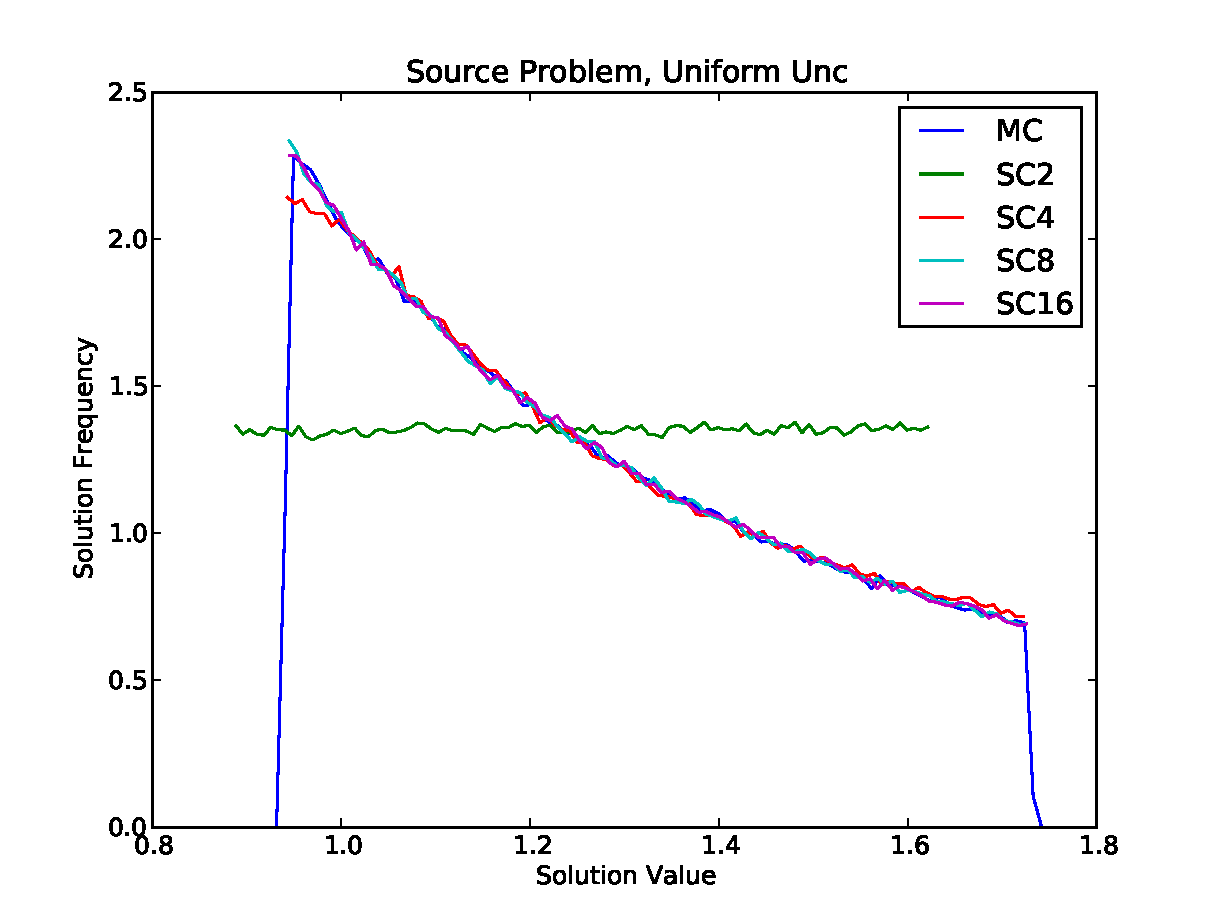
\includegraphics[width=\textwidth]{../graphics/source_uniform_pdfs}
   \caption{Uniform}
      \label{uni}
  \end{subfigure}
  \begin{subfigure}[b]{0.45\textwidth}
   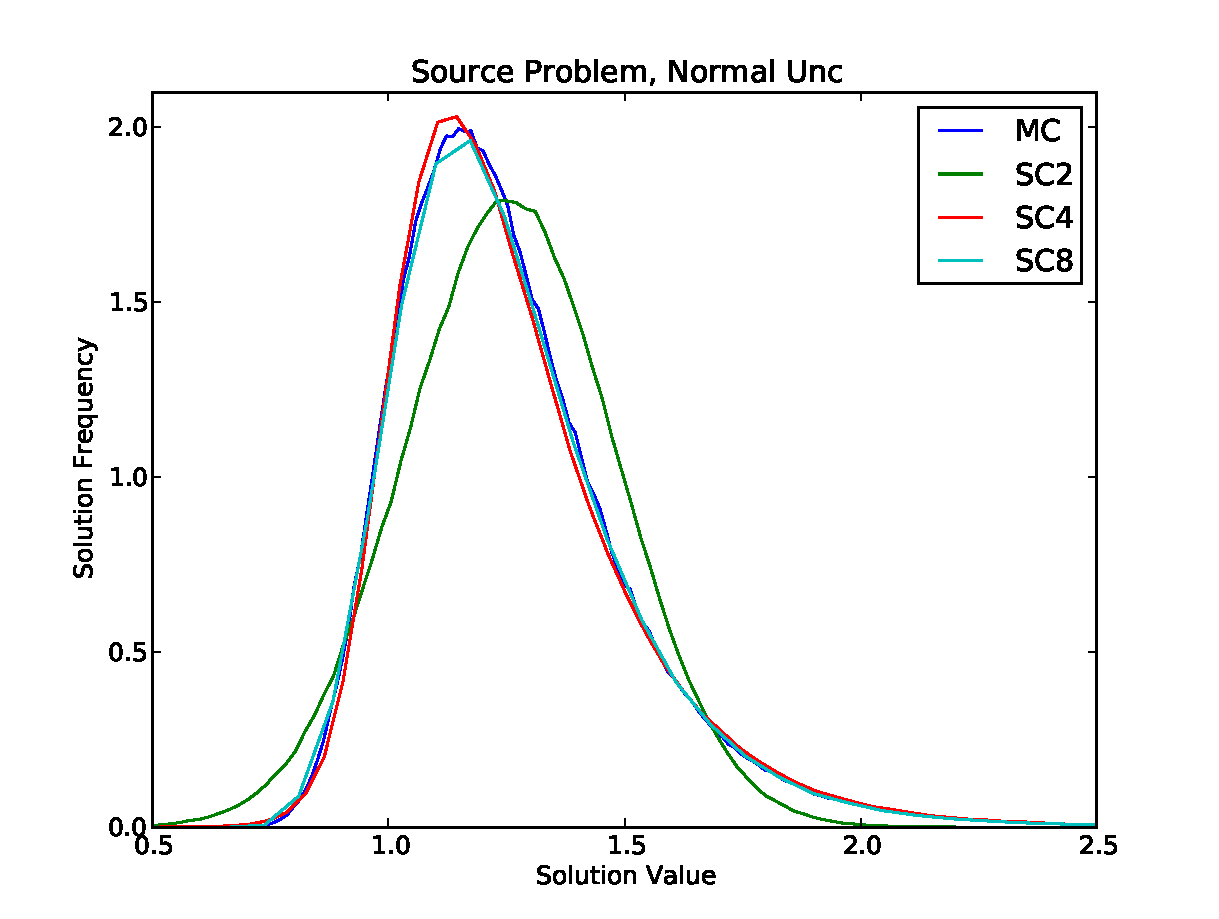
\includegraphics[width=\textwidth]{../graphics/source_normal_pdfs}
   \caption{Normal}
      \label{norm}
  \end{subfigure}
\caption{Univariate Source Solver PDFs}
\label{fig:source uni res}
\end{figure}

\subsection{1D Diffusion Solver: $k=k\qty(D_g,\Sigma_{g,c},\Sigma_{g'\to g,s},\Sigma_{g,f},\nu_g)$}
For the univariate case, we introduce uncertainty in the neutron capture cross section of the second energy group $\Sigma_{2,c}$.   We consider three cases, $\Sigma_{2,c}$ distributed normally in each.  We choose a different mean for each distribution.  Each mean corresponds to a different reactivity state: subcritical, critical, and supercritical ($k=(0.9,1.0,1.1)$).  The three distributions are respectively $\Sigma_{2,c}\sim\qty(\mathcal{N}(0.055969,0.1),\mathcal{N}(0.04438,0.1),\mathcal{N}(0.035181,0.1))$.  We also restrict Monte Carlo sampling of the uncertain parameter to three standard deviations around the mean, effectively creating a truncated normal distribution.  For this reason, the mean and variance of the Monte Carlo sampling do not converge on the analytic values.  The results are shown in Table \ref{tab: 1d uni res}.  The solution PDFs are shown in Fig. \ref{fig:1d uni res}.
\begin{table}[H]
\begin{center}
\begin{tabular}{c|c c|l l}
Type & UQ & runs$|$order & mean & variance \\ \hline
Subcritical & MC & $1\times10^6$ & 0.907699673282 & 0.00632790358771 \\
&SC & 2 & 0.907653521565 & 0.00595095987773 \\
&SC & 4 & 0.907813174929 & 0.00633526057266\\
&SC & 8 & 0.907813389468 & 0.00633649118503 \\
&SC & 16 & 0.907813389471 & 0.00633649126226 \\ \hline
Critical &MC & $1\times10^6$ & 1.01144778738 & 0.0105716289269   \\
&SC & 2 & 1.01107577584 & 0.00974910361412  \\
&SC & 4 & 1.0113755955 & 0.0105739848126 \\
&SC & 8 & 1.01137628238 & 0.0105785232446 \\
&SC & 16 & 1.01137628243 & 0.0105785241745 \\ \hline
Supercritical & MC & $1\times10^6$ & 1.11593980088 & 0.0168503796482 \\
&SC & 2 & 1.11537873568 & 0.0151539223359 \\
&SC & 4 & 1.11590698755 & 0.016795821961\\
&SC & 8 & 1.11590896034 & 0.0168106966474 \\
&SC & 16 & 1.11590896088 & 0.0168107061554
\end{tabular}
\end{center}
\caption{1D Solver, Univariate Statistics}
\label{tab: 1d uni res}
\end{table}

\begin{figure}[h!]
\centering
   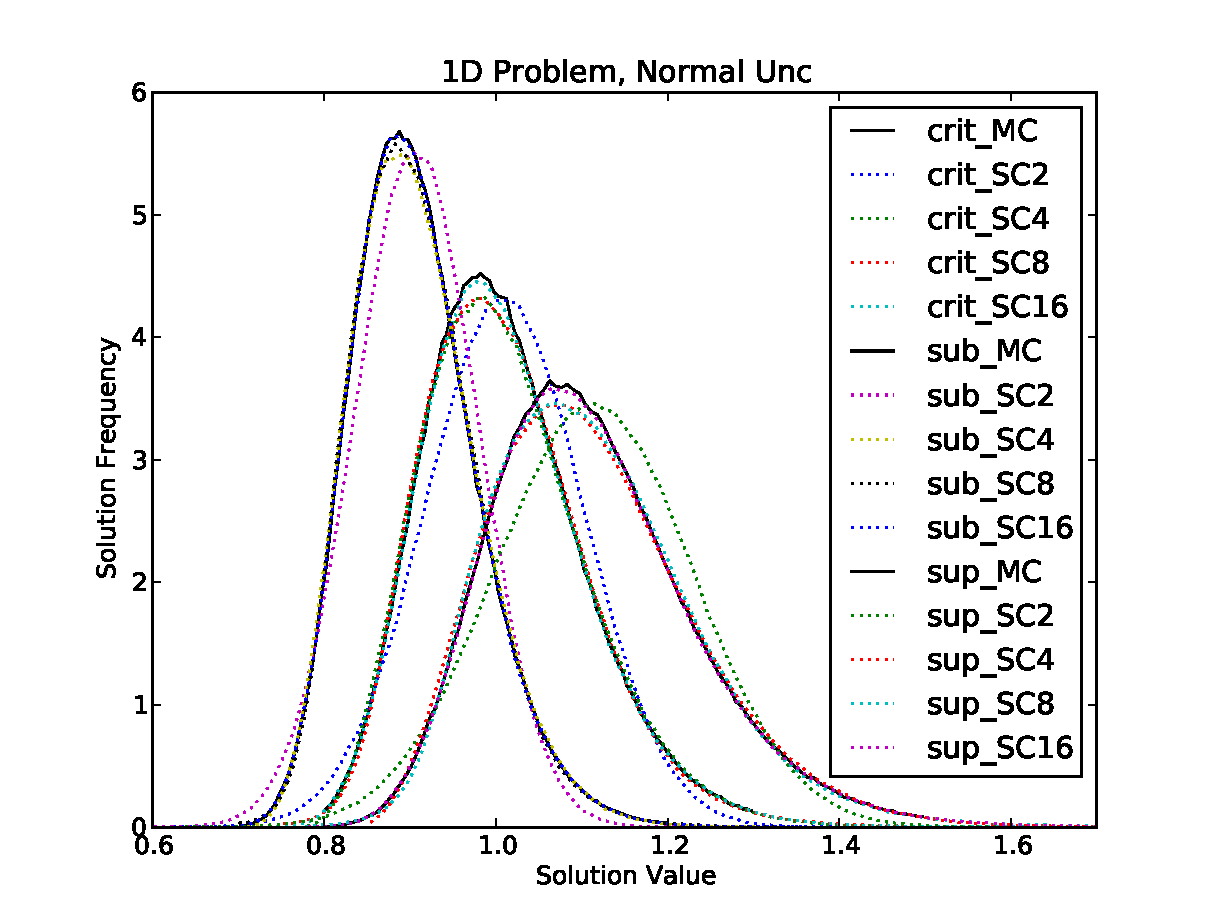
\includegraphics[width=.75\textwidth]{../graphics/1dall_normal_pdfs}
   \caption{Univariate 1D Solver PDFs}
   \label{fig:1d uni res}
\end{figure}


\newpage
\subsection{Quarter Core Solver: $k=k\qty(D_g^{(R)},\xs{g,c}{R},\xs{g'\to g,s}{R},\xs{g,f}{R},\nu_g^{(R)})$}
The original benchmark parameters before introducing uncertainty are in Table \ref{tab:coremats}.
\begin{figure}[H]
\centering
   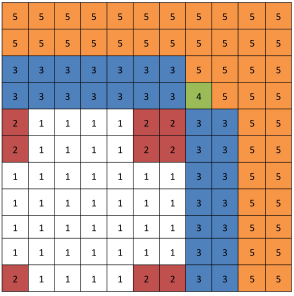
\includegraphics[width=0.4\textwidth]{../graphics/core}
   \caption{Quarter Core Map}
\end{figure}
\begin{table}[H]
\centering
\begin{tabular}{c c | c c c c}
Material (R)& Group & $D_g^{(R)}$ & $\xs{g,c}{R}$ & $\nu\xs{g,f}{R}$ & $\xs{1\to2,s}{R}$ \\ \hline
1 & 1 & 1.255    & 4.602e-3 & 4.602e-3 & 2.533e-2 \\
  & 2 & 2.11e-1  & 5.540e-2 & 1.091e-1 & \\ \hline
2 & 1 & 1.268    & 4.609e-3 & 4.609e-3 & 2.767e-2 \\
  & 2 & 1.902e-1 & 8.675e-2 & 8.675e-2 & \\ \hline
3 & 1 & 1.259    & 6.083e-3 & 4.663e-3 & 2.617e-2 \\
  & 2 & 2.091e-1 & 4.142e-2 & 1.021e-1 & \\ \hline
4 & 1 & 1.259    & 4.663e-3 & 4.663e-3 & 2.617e-2 \\
  & 2 & 2.091e-1 & 3.131e-2 & 1.021e-1 & \\ \hline
5 & 1 & 1.257    & 6.034e-4  & 0 & 4.754e-2 \\
  & 2 & 1.592e-1 & 1.911e-2  & 0 & 
\end{tabular}
\caption{Material Properties for Core}
\label{tab:coremats}
\end{table}
Similar to the one-dimensional problem, we introduce uncertainty in the low-energy capture cross section, in this case only in Material 1 $\qty(\xs{2,c}{1})$, which makes up the majority of the core.  We consider two distributions, $\xs{2,c}{1}\sim\qty(\mathcal{U}(0.0454,0.0654),\mathcal{N}(0.0554,0.01^2))$.  Because of the nonlinear dependence of the solution on the input parameter, we use order 32 Gauss quadrature to obtain all the polynomial expansion coefficients, instead of scaling them with the total expansion order.  The Monte Carlo sampling algorithm rejects samples outside three standard deviations, causing discrepancy in the mean and variance.
\begin{table}[H]
\begin{center}
\begin{tabular}{c|c c|l l}
Type & UQ & runs$|$order & mean & variance \\ \hline
Uniform &MC & $1\times10^6$ & 1.00406413634 & 0.000446173081079 \\
&SC & 2  & 1.00416405471 & 0.000375112851817 \\
&SC & 4  & 1.00416405471 & 0.000390962150246 \\
&SC & 8  & 1.00416405471 & 0.000406864600682 \\
&SC & 16 & 1.00416405471 & 0.000421349517322 \\
&SC & 32 & 1.00416405471 & 0.000425027572716 \\ \hline
Normal &MC & $1\times10^6$ & 1.01333702129 & 0.00160652595587 \\
&SC & 2  & 1.01643813464 & 0.00138703446968 \\
&SC & 4  & 1.01643813464 & 0.00184314998697 \\
&SC & 8  & 1.01643813464 & 0.00184690058216 \\
&SC & 16 & 1.01643813464 & 0.00184724103523 \\
&SC & 32 & 1.01643813464 & 0.00184726152781
\end{tabular}
\end{center}
\caption{Quarter Core Solver, Univariate Statistics}
\label{tab: 2d uni res}
\end{table}

%\begin{figure}[h]
%\centering
%  \begin{subfigure}[b]{0.45 \textwidth}
%   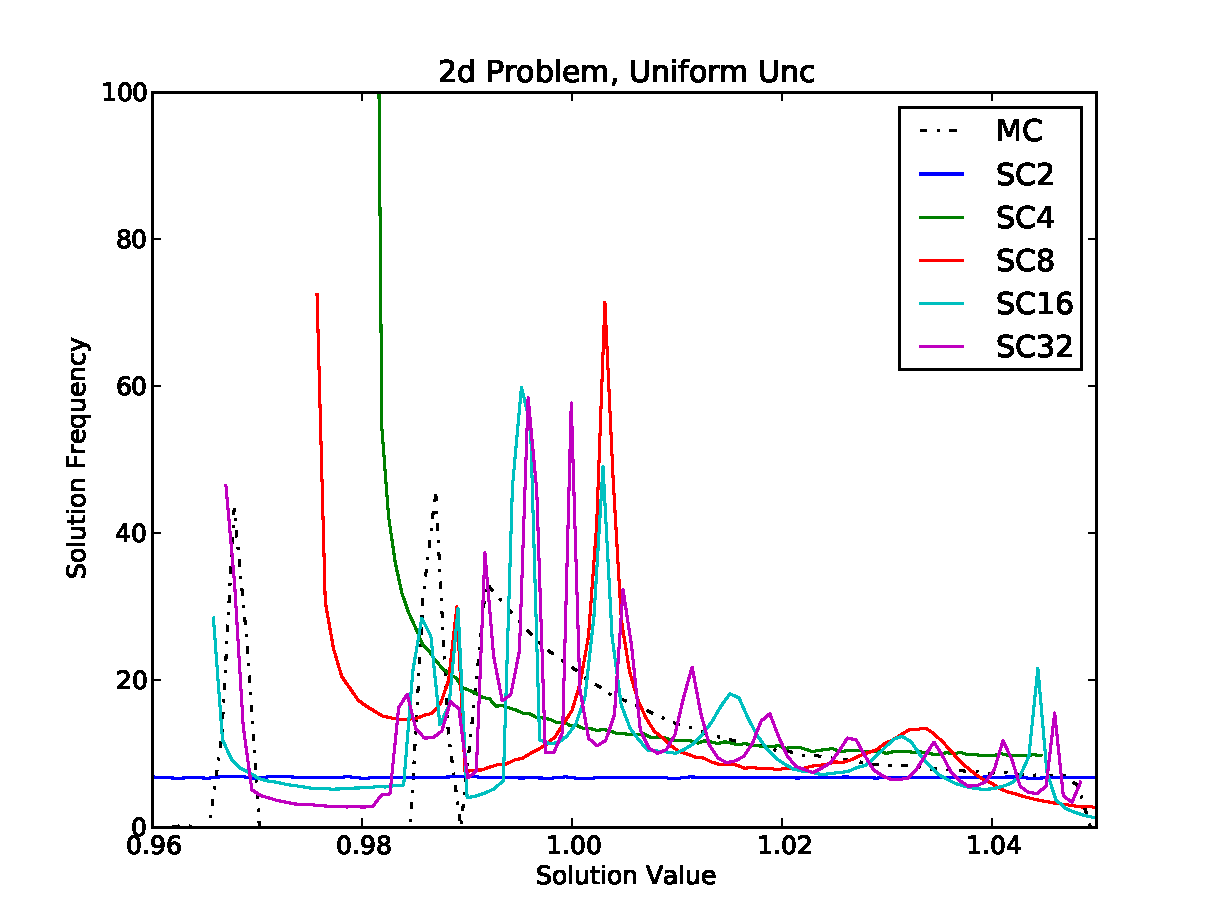
\includegraphics[width=\textwidth]{../graphics/2d_uniform_pdfs}
%   \caption{Uniform}
%      \label{uni}
%  \end{subfigure}
%  \begin{subfigure}[b]{0.45\textwidth}
%   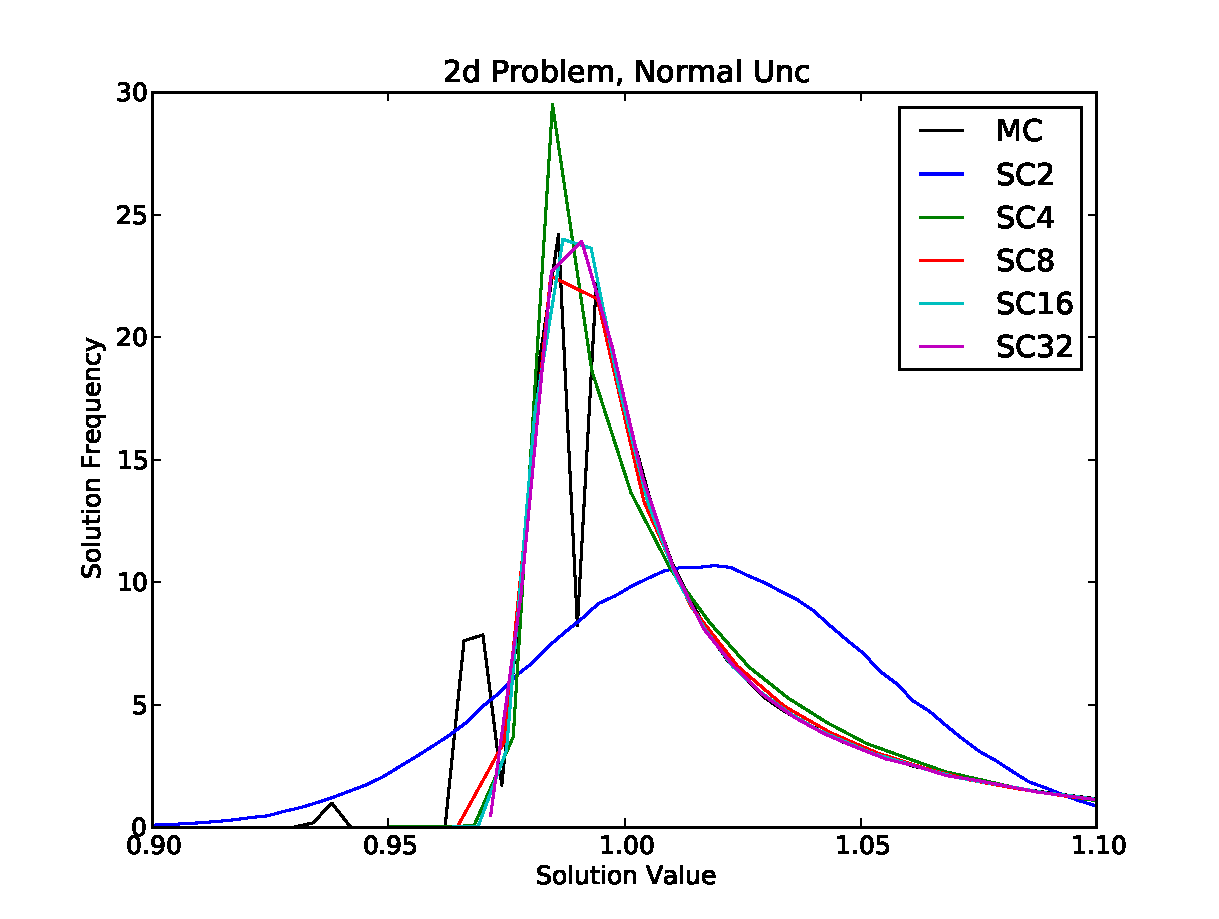
\includegraphics[width=\textwidth]{../graphics/2d_normal_pdfs}
%   \caption{Normal}
%      \label{norm}
%  \end{subfigure}
%\caption{Univariate Quarter Core Solver PDFs}
%\label{fig:source uni res}
%\end{figure}
\begin{figure}[H]
\centering
   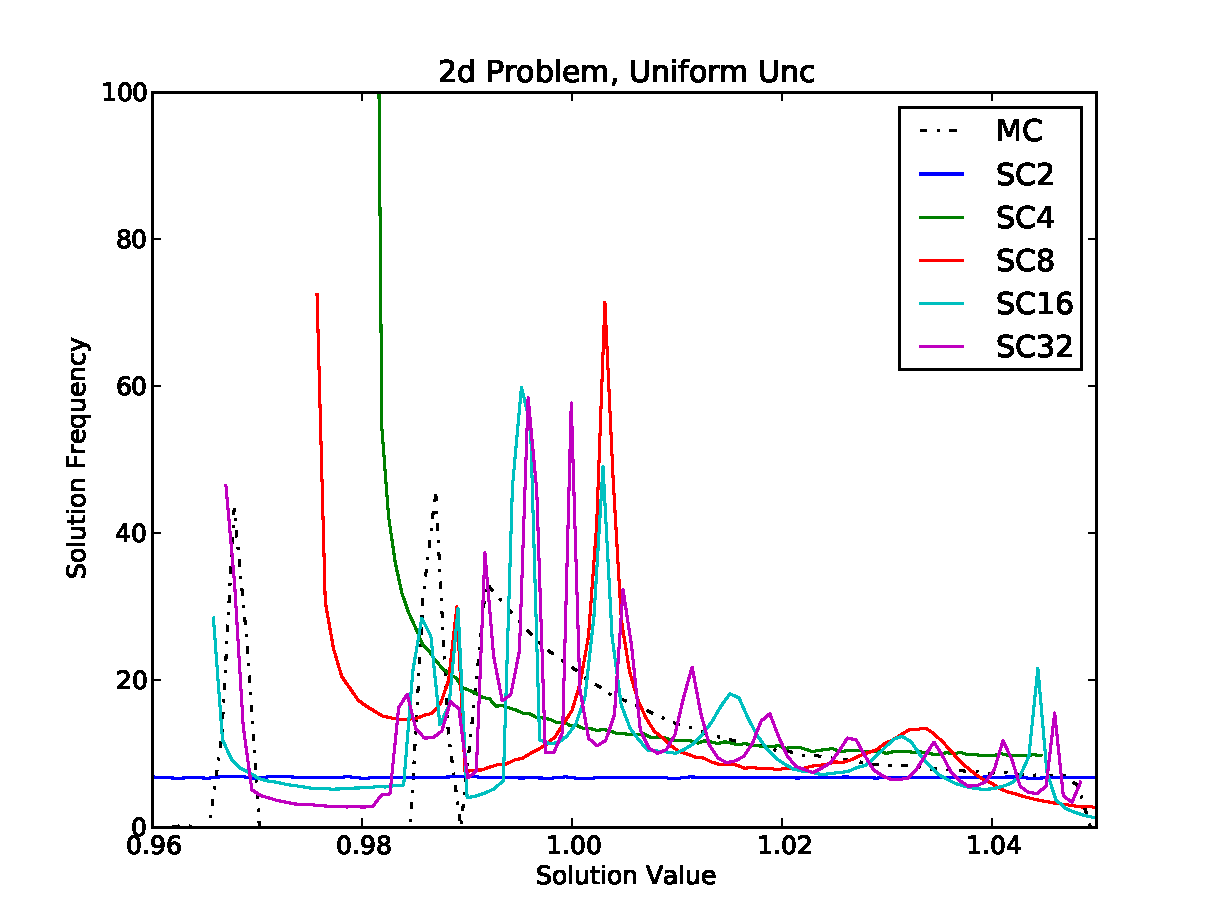
\includegraphics[width=0.7\textwidth]{../graphics/2d_uniform_pdfs}
   \caption{Uniform Univariate Quarter Core Solver PDFs}
   \label{fig:2dcrit uni}
\end{figure}
\begin{figure}[H]
\centering
   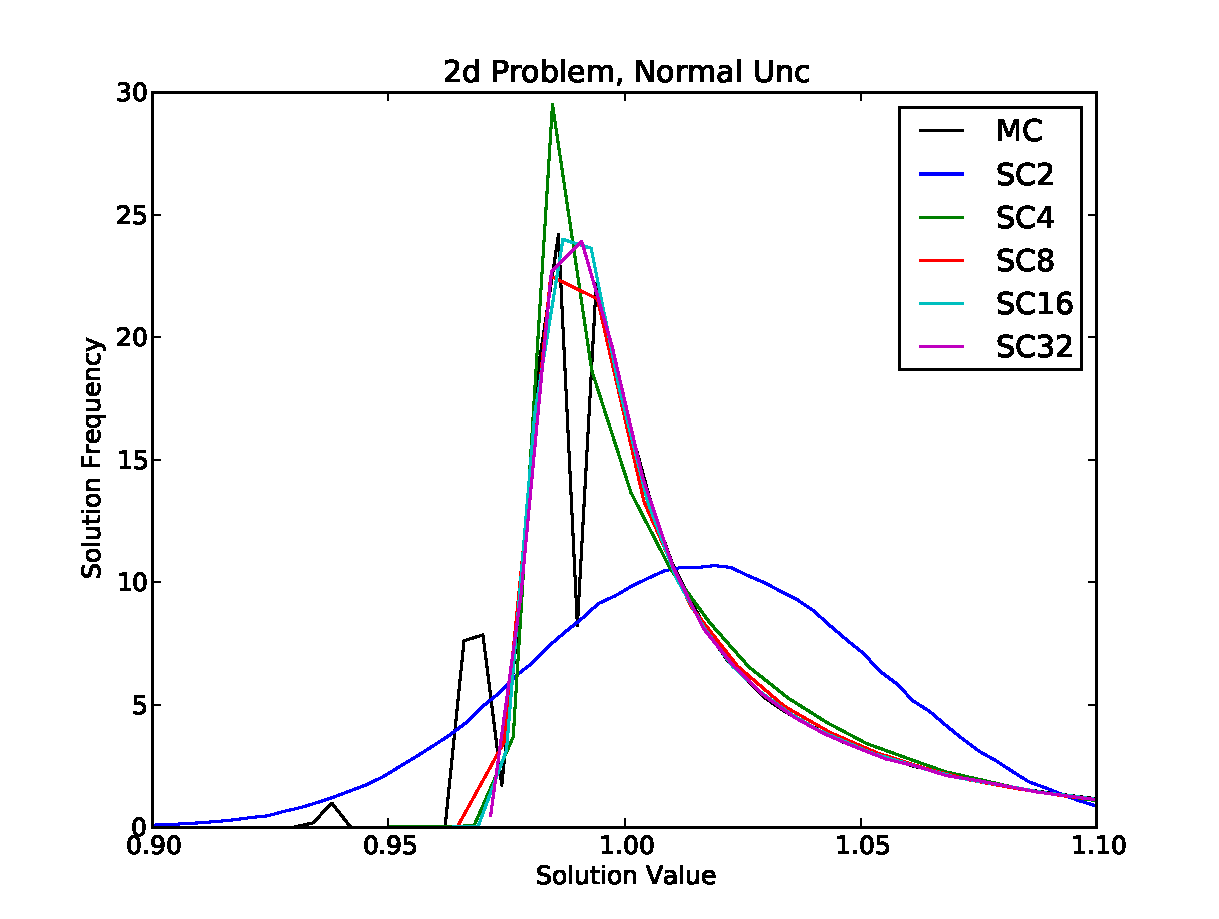
\includegraphics[width=0.7\textwidth]{../graphics/2d_normal_pdfs}
   \caption{Normal Univariate Quarter Core Solver PDFs}
   \label{fig:2dcrit}
\end{figure}

\section{Convergence}
There are several factors that contribute to the successful convergence of the polynomial chaos expansion sum with coefficients calculated by quadrature.  The coefficients are calculated as
\begin{equation}
u_p \approx \sum_{\ell=0}^{L} w_\ell U(Y_\ell) \psi_p(Y_\ell).
\end{equation}
Two significant sources of error appear in this calculation: first, the quadrature truncation error from using only $L$ terms in the quadrature set; second, the inherent error in the solver $U(Y)$, which we denote spatial discretization error.  While this assumes the error in the solver is chiefly from the division of the domain into a mesh of finite refinement (for example, using finite element or finite volume methods), it could similarly apply to other solution method errors.
We consider the impact of both quadrature truncation error and spatial discretization error on the convergence of the expansion coefficients.

\subsection{Quadrature}\label{sec:quadconv}
One concern with using stochastic collocation to build the polynomial chaos moments is the appropriate order of quadrature to use.  With Gaussian quadrature, a sum with $n$ terms can exactly integrate a polynomial of order $2n-1$.  The chaos moment expression we integrate is
\begin{align}
u_p &= \int_\Omega U(Y)\rho(Y)\psi_p(Y)dY,\\
  &\approx \sum_{\ell=0}^L w_\ell U(Y_\ell)\psi_p(Y_\ell),
\end{align}
where $\rho$ is the probability distribution of $Y$ and $\psi_p$ is the $p-th$ order basis polynomial.  In the simplest case when $U(Y)$ is a scalar quantity, the order of the expression under the integral is determined solely by the basis polynomial.  Thus a quadrature order of $(i+1)/2$ is the minimum quadrature order necessary to integrate the chaos moments.  In the case $U(Y)$ is highly nonlinear and ill-approximated by even high-order polynomials, the necessary quadrature order required to accurately determine moments is much higher.

As an example of chaos moment convergence as a function of quadrature order, we show the PCESC moments of the 1D diffusion solver critical case for 7th-order quadrature in Table \ref{tab:quadconverge}, as determined by increasing orders of quadrature from the minimum to 12-th order, which assumes $U(Y)$ alone is well-approximated by a 7th-order polynomial.  As can be seen, the lower moments require smaller quadrature orders, and at least order 8 quadrature is necessary to see reasonable convergence for higher moments.  While the mean converges with low-order quadrature, the highest expansion order doesn't converge to discretization error until 10-th order quadrature is used.

Table \ref{tab:1dcrit coeffs} shows expansion moments calculated using quadrature order equal to expansion order for orders up through 31.


\begin{landscape}
\begin{table}[H]
\begin{center}
\begin{tabular}{c | *{8}{l}}
Quadrature Order & $u_0$ & $u_1$ & $u_2$ & $u_3$ & $u_4$ & $u_5$ & $u_6$ & $u_7$ \\ \hline
5 & 1.34648094 & -0.13502447 & 0.02226791 & -0.0045477 & 0.00000000 & 0.00101863 & -0.00092988 & 0.00313821\\
6 & 1.34648100 & -0.13502501 & 0.02227125 & -0.00456451 & 0.0010908 & -0.00027317 &  0.00000000 & 0.00025291\\ 
8 & 1.34648101 & -0.13502506 & 0.02227158 & -0.00456614 & 0.0010978 & -0.00029964 & 9.01120742e-05 & -2.67010906e-05\\ 
10& 1.34648101 & -0.13502506 & 0.02227158 & -0.00456616 & 0.0010979 & -0.00030000 & 9.13419949e-05 & -3.05173759e-05\\ 
12& 1.34648101 & -0.13502506 & 0.02227158 & -0.00456616 & 0.0010979 & -0.00030001 & 9.13732306e-05 & -3.06142832e-05
\end{tabular}
\end{center}
\caption{Chaos Moment Convergence with Increasing Quadrature Order}
\label{tab:quadconverge}
\end{table}
\end{landscape}

\begin{table}[H]
\begin{center}
\begin{tabular}{c | l l l l l}
Moment & SC1 & SC3 & SC7 & SC15 & SC31\\ \hline
0 & 1.34608094 & 1.3464801 & 1.34648101 & 1.34648101 &  1.34648101\\
1 & -0.13145279 & -0.1350169 & -0.13502506 & -0.13502506 &  -0.13502506\\ 
2 & 0 & 0.02222067 & 0.02227158 & 0.02227158 &  0.02227158\\ 
3 & 0 & -0.00431037 & -0.00456614 & -0.00456616 & -0.00456616 \\ 
4 & 0 & 0 & 0.0010978 & 0.0010979 & 0.0010979 \\ 
5 & 0 & 0 & -0.00029964 & -0.00030001 & -0.00030001 \\ 
6 & 0 & 0 & 9.01120742e-05 & 9.13747084e-05 & 9.13746830e-05 \\ 
7 & 0 & 0 & -2.67010906e-05 & -3.06188612e-05 & -3.06187650e-05 \\ 
8 & 0 & 0 & 0 & 1.11868181e-05 & 1.11865704e-05 \\ 
9 & 0 & 0 & 0 & -4.42800671e-06 & -4.42735312e-06 \\ 
10 & 0 & 0 & 0 & 1.89021407e-06 & 1.88853134e-06 \\ 
11 & 0 & 0 & 0 & -8.66874281e-07 & -8.62852707e-07 \\ 
12 & 0 & 0 & 0 & 4.24658199e-07 & 4.15693998e-07 \\ 
13 & 0 & 0 & 0 & -2.18790217e-07 & -1.99976426e-07 \\ 
14 & 0 & 0 & 0 & 1.12938059e-07 & 7.56801496e-08 \\ 
15 & 0 & 0 & 0 & -4.90000878e-08 & 2.05894301e-08 \\ 
16 & 0 & 0 & 0 & 0 & -1.22580841e-07 \\ 
17 & 0 & 0 & 0 & 0 & 2.51097599e-07 \\ 
18 & 0 & 0 & 0 & 0 & -4.18278488e-07 \\ 
19 & 0 & 0 & 0 & 0 & 6.25910592e-07 \\ 
20 & 0 & 0 & 0 & 0 & -8.61060458e-07 \\ 
21 & 0 & 0 & 0 & 0 & 1.09209939e-06 \\ 
22 & 0 & 0 & 0 & 0 & -1.26866179e-06 \\ 
23 & 0 & 0 & 0 & 0 & 1.32892404e-06 \\ 
24 & 0 & 0 & 0 & 0 & -1.21597330e-06 \\ 
25 & 0 & 0 & 0 & 0 & 9.01437926e-07 \\ 
26 & 0 & 0 & 0 & 0 & -4.09433059e-07 \\ 
27 & 0 & 0 & 0 & 0 & -1.70599526e-07 \\ 
28 & 0 & 0 & 0 & 0 & 6.94034499e-07 \\ 
29 & 0 & 0 & 0 & 0 & -9.99892578e-07 \\ 
30 & 0 & 0 & 0 & 0 & 9.71463606e-07 \\ 
31 & 0 & 0 & 0 & 0 & -5.97051529e-07 \\ 
\end{tabular}
\end{center}
\caption{Chaos Moments for 1D Critical Case}
\label{tab:1dcrit coeffs}
\end{table}


\newpage
\subsection{Spatial Discritization}\label{sec:spaceconv}
To see the effect of spatial discretization on coefficient convergence, we consider the quarter core benchmark solver.  We consider five univariate cases.  In each, we vary a different parameter chosen from $\xs{2,c}{1},\xs{2,f}{1},\xs{2,c}{4},\xs{2,f}{4},D_{2}^{(5)}$.  For each parameter, we use the coarsest mesh (11x11) possible in the quarter-core benchmark and plot the expansion coefficients up to order 256, shown in Fig. \ref{fig:2g2d5v coarse cof}.  While the Material 4 and Material 5 properties converge quickly to acceptable levels, the Material 1 properties fail to converge past a magnitude of $10^{-4}$.
\begin{figure}[H]
\centering
   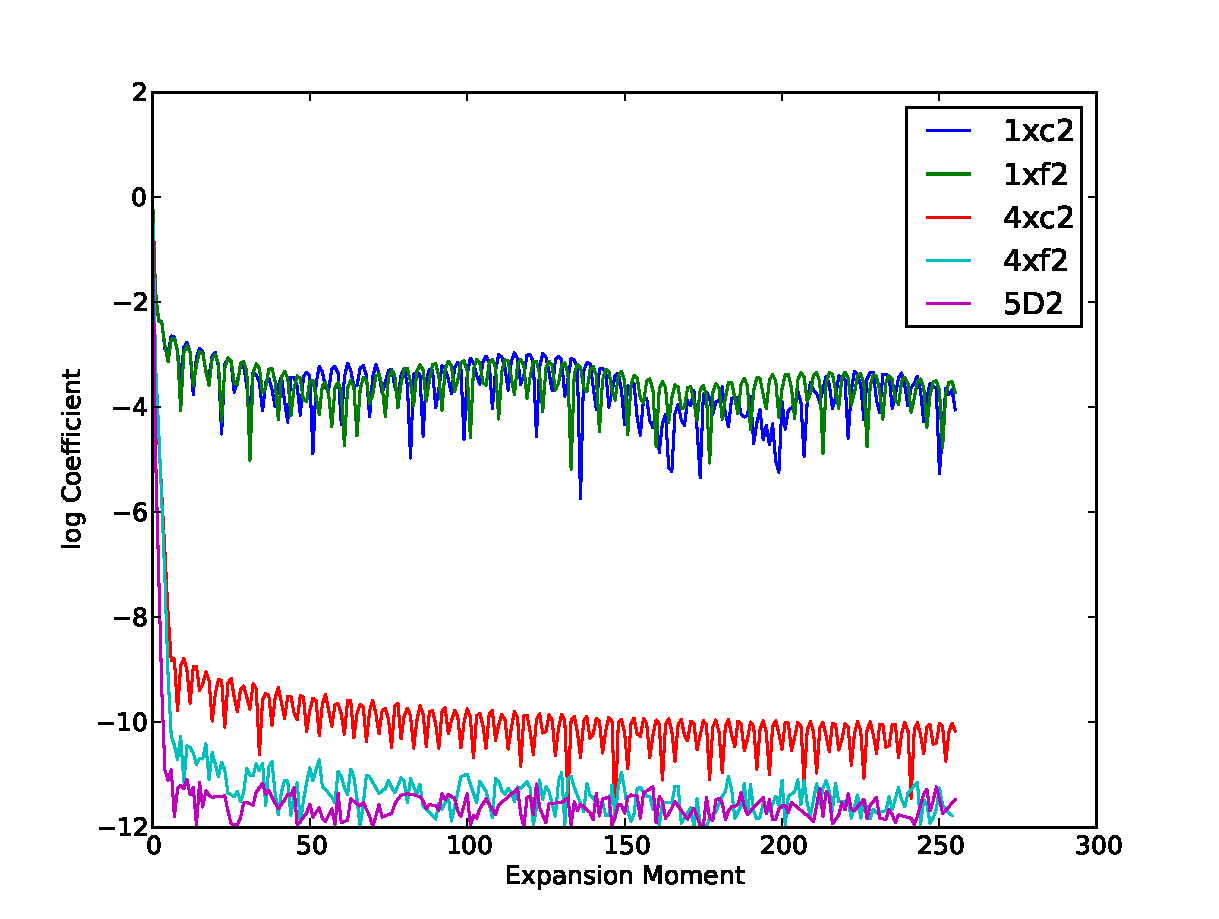
\includegraphics[width=0.7\textwidth]{../graphics/coefficient_decay}
   \caption{Quarter Core Solver Coarse Mesh Coefficient Decay}
   \label{fig:2g2d5v coarse cof}
\end{figure}
To demonstrate the effect of increasing mesh refinement, we consider only the low-energy capture cross section for the first region (1xc2, $\xs{2,c}{1}$).  In each successive refinement $n=(1,2,3,4,5)$ we subdivide each of the 121 regions of the problem into $n^2$ cells, so that for $n=2$ the global mesh is 22x22, and so on.  The results are shown in Fig. \ref{fig:2g2d 1xc2 cof decay}.  With only one additional refinement level, the coefficients converge to acceptable levels.
\begin{figure}[H]
\centering
   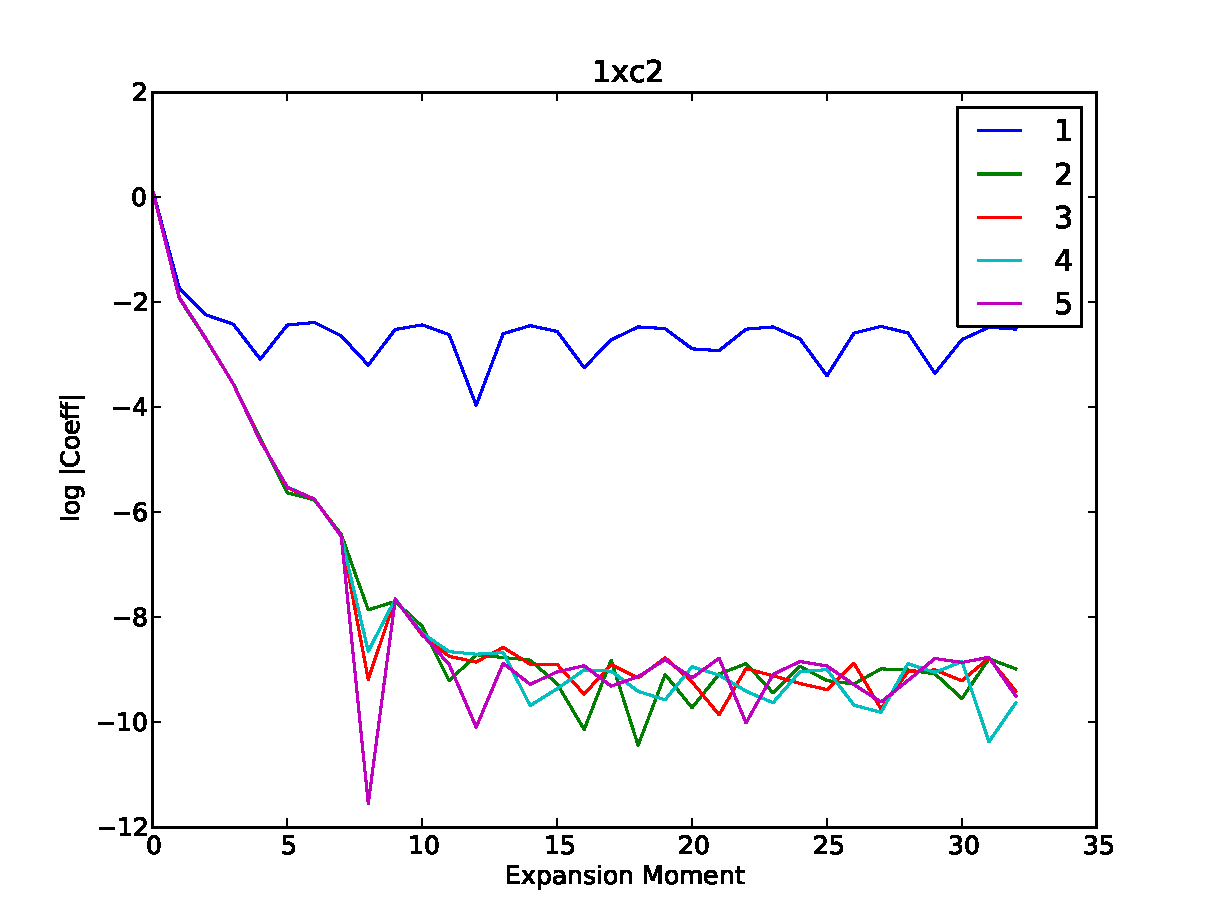
\includegraphics[width=0.7\textwidth]{../graphics/cof_decay_1xc2_meshes}
   \caption{2G2D: Coefficients over Mesh Refinement}
   \label{fig:2g2d 1xc2 cof decay}
\end{figure}
We repeat the original exercise, this time making use of the $n=2$ refined mesh, and see all coefficients converging to an acceptable level after several terms.  The results are in Fig. \ref{fig:2g2d5v fine cof}.
\begin{figure}[H]
\centering
   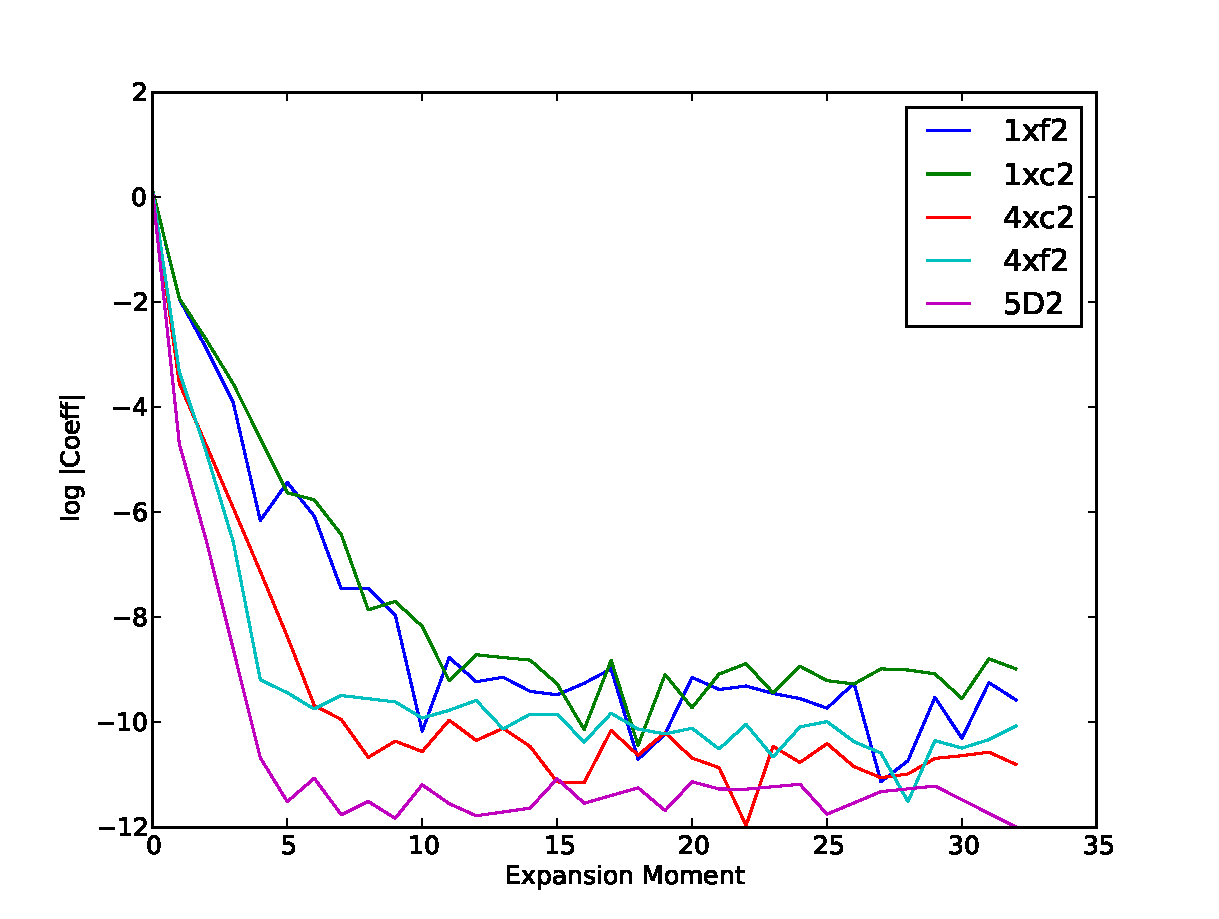
\includegraphics[width=0.7\textwidth]{../graphics/coefficient_decay2}
   \caption{2G2D: Coarse Mesh Coefficient Decay}
   \label{fig:2g2d5v fine cof}
\end{figure}
\section{Multivariate UQ}
We now extend the univariate uncertainty quantification to multivariate solvers.  For now, we limit ourselves to the tensor product collocation space, which we acknowledge as sufficient but quite inefficient.  Improving on this approach is the significant focus for future work.  We consider uncertain vector $Y=[Y_1,Y_2,\ldots,Y_N]$ as uncertain input parameters for the solution $U(Y)$.  We expand as before, but considering $N$ uncorrelated input parameters:
\begin{equation}
U(\theta;Y)\approx U_P(\theta;Y) = \sum_{p_1=0}^{P_1}\sum_{p_2=0}^{P_2}\cdots\sum_{p_N=0}^{P_N} u_{\bar p}(\theta) \prod_{n=1}^N\psi_{p_n}(Y),
\end{equation}
where now multi-index $\bar p=[p_1,p_2,\ldots,p_N]$ denotes a single set of expansion orders, one for each variable.  The multi-index is taken from the multi-index set $\Lambda(L)$, which includes all desired multi-indices.  In the case of tensor product space,
\begin{equation}
\Lambda_\text{TP}(L)=\qty{\bar p=(p_1,\ldots,p_N):\max_{1\leq n\leq N} P_n\leq L}.
\end{equation}
This tensor product space quickly becomes unmanageably large, as the size of the index set scales as
\begin{equation}
|\Lambda_\text{TP}(L)|=(L+1)^N.
\end{equation}
However, this index set will serve to demonstrate the UQ algorithm and its capacity to treat multivariate UQ for deterministic solvers.

\subsection{Polynomial Solver: $f(x,y)$}
We once again include this case for its analytic mean and variance.  We introduce uniform uncertainty to both parameters as $x\sim\mathcal{U}(3,7),y\sim\mathcal{U}(1,6)$.  The analytic expected statistics along with the Monte Carlo and PCESC statistics are shown in Table \ref{tab: poly milt res}, and the PDFs in Fig. \ref{fig: poly milt res}
\begin{table}[H]
\begin{center}
\begin{tabular}{c c|l l}
type & runs/order & mean & variance \\ \hline
Analytic & - & $45/2$ & $81.8611111111$ \\
MC & $1\times10^7$ & 22.4962950638 & 81.8754664265 \\
SC & (1,1) & 22.5 & 81.8611111111 \\
\end{tabular}
\end{center}
\caption{Polynomial Solver, Bivariate Uniform Distribution Statistics}
\label{tab: poly milt res}
\end{table}
\begin{figure}[H]
\centering
%  \begin{subfigure}[b]{0.45 \textwidth}
   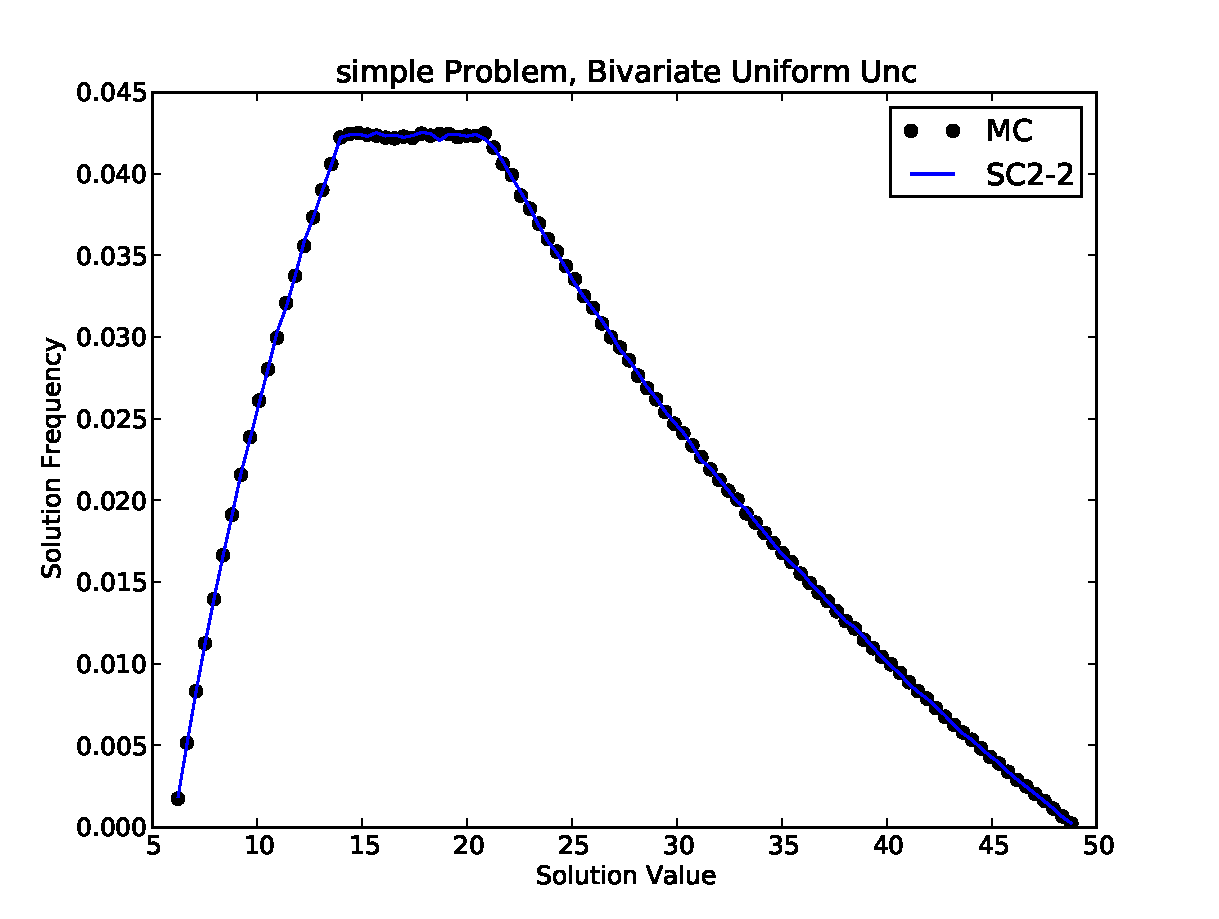
\includegraphics[width=0.5\textwidth]{../graphics/poly_2v_uniform_pdfs}
   \caption{Polynomial Solver, Bivariate Uniform PDFs}
      \label{fig: poly milt res}
%  \end{subfigure}
\end{figure}

\subsection{Source Solver: $\phi=\phi\qty(S,D,x,\Sigma_a)$}
In addition to the absorption cross section, we introduce uncertainty in the location at which the flux is measured.  This occasion might arise when the exact absorption properties of a medium are unknown and a point detector is placed with some uncertainty.  We allow the input parameters to be uncertain as $\Sigma_a\sim\mathcal{U}(0.5,1),x\sim\mathcal{U}(1.5,2.5)$.  The other two parameters remain constant as
\begin{align}
S &= 1.0 \text{ n/cm}^2\text{/s},\\
D &= 0.5 \text{ /cm}.
\end{align}
The statistical results are in Table \ref{tab: source mult res} and the PDFs in Fig. \ref{fig: source mult res}.
\begin{table}[H]
\begin{center}
\begin{tabular}{c c|l l}
type & order($\Sigma_a,x$) & mean & variance \\ \hline
MC & $1\times10^6$ & 1.24791828682 & 0.0508287413676\\
SC & (2,2) & 1.24804231569 & 0.0506451101763 \\
SC & (2,4) & 1.24804212351 & 0.0506466208388\\
SC & (4,2) & 1.24806746049 & 0.0507934845282\\
SC & (4,4) & 1.24806726831 & 0.0507949951904 \\
\end{tabular}
\end{center}
\caption{Statistics for Source Solver with Bivariate Uniform Uncertainty}
\label{tab: source mult res}
\end{table}
\begin{figure}[h]
\centering
   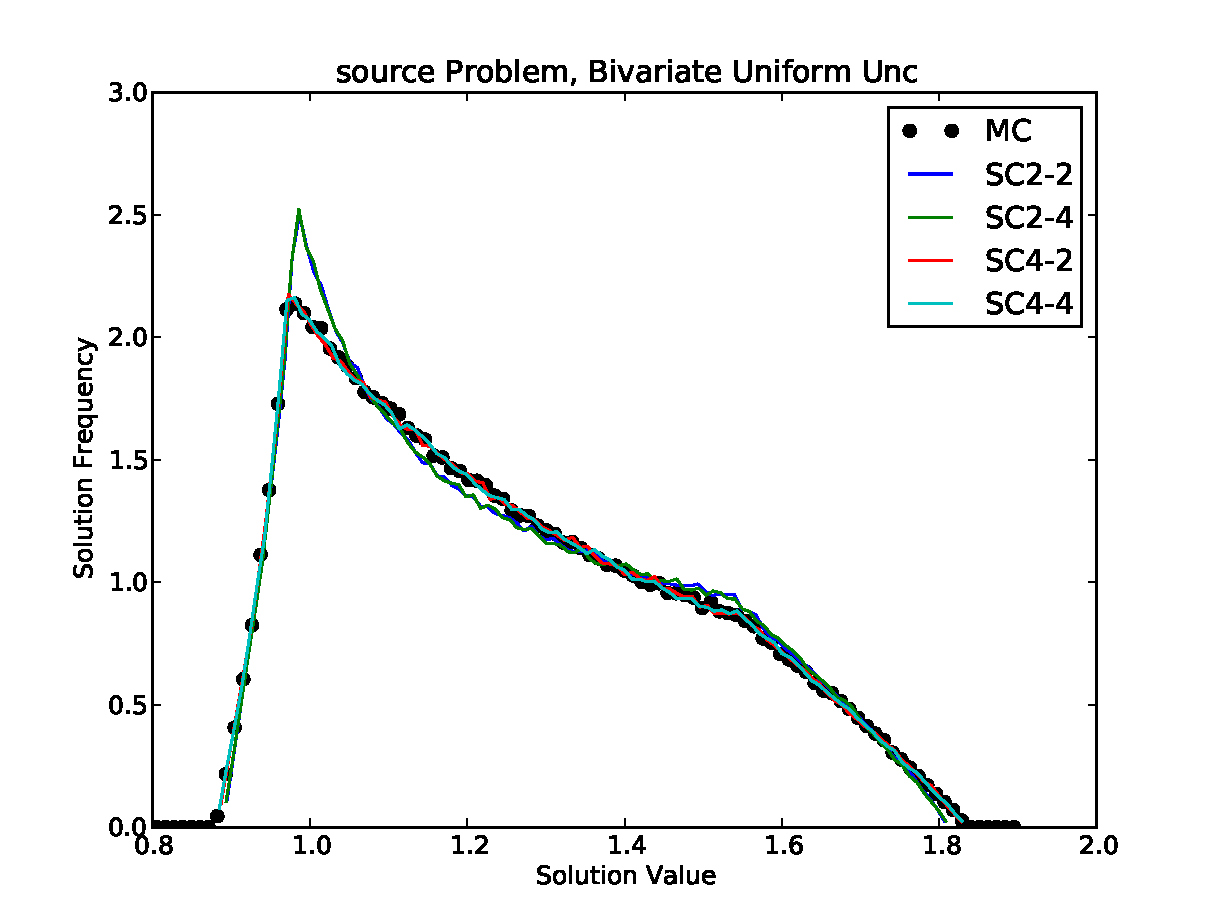
\includegraphics[width=0.5\textwidth]{../graphics/source_2v_uniform_pdfs}
\caption{Bivariate Source Solver Solution Distributions}
\label{fig: source mult res}
\end{figure}

\newpage
\subsection{Quarter Core Solver: $k=k\qty(D_g^{(R)},\xs{g,c}{R},\xs{g'\to g,s}{R},\xs{g,f}{R},\nu_g^{(R)})$}
In this case we consider five uncertain parameters simultaneously, as in Table \ref{tab:2d2g5param}.  Each was given approximately 10\% uncertainty from its mean in the benchmark problem.
\begin{table}[H]
\begin{center}
\begin{tabular}{c c c c}
Region & Energy Group & Parameter & Uncertainty \\ \hline
1 & 2 & $\Sigma_c$ & $\mathcal{U}(0.050,0.061) $\\
1 & 2 & $\Sigma_f$ & $\mathcal{U}(0.098,0.120) $\\
4 & 2 & $\Sigma_c$ & $\mathcal{U}(0.037,0.046) $\\
4 & 2 & $\Sigma_f$ & $\mathcal{U}(0.092,0.112) $\\
5 & 2 & $D$            & $\mathcal{U}(0.143,0.175) $\\
\end{tabular}
\end{center}
\caption{Quarter Core Multivariate Uncertainty Space}
\label{tab:2d2g5param}
\end{table}

We also can attempt to make informed guesses as to the appropriate expansion order of each input parameter by performing independent convergence studies for each.  Using the results from \S \ref{sec:spaceconv}, we use expansion orders based on convergence tolerance.  The results are in Table \ref{tab:2dcrit5v}.

\begin{table}[H]
\begin{center}
\begin{tabular}{c c c|l l}
type & tol & $\mathcal{P}(\Sigma_{2,c}^1,\Sigma_{2,f}^1,\Sigma_{2,c}^4,\Sigma_{2,f}^4,D^5_2)$ & mean & variance \\ \hline
MC & - & - & 0.999064586714 & 0.0262019588485 \\
SC & 1e-4 & (5, 4, 3, 3, 1) & 1.00191085676 & 0.000202816510815 \\
SC & 1e-5 & (6, 5, 4, 3, 1) & 1.00112487809 & 0.000554497293737\\
SC & 1e-6 & (8, 7, 5, 4, 2) & 1.00018130781 & 0.00245280240592 \\
SC & 1e-8 & (10, 9, 6, 4, 3) & 1.00014901416 & 0.00207327774315
\end{tabular}
\end{center}
\caption{Statistics for Multivariate Quarter Core Solver}
\label{tab:2dcrit5v}
\end{table}
The mean is converged quite swiftly.  The variance improves quickly with decreased tolerance, but there is still an order of magnitude difference between the Monte Carlo-calculated variance and the PCESC-calculated variance.  This suggests that considering only independent convergence of parameters is insufficient, and future studies will include consideration for convergence by pairwise input parameters.

\section{Index Sets}
In the previous section, we use coefficients for the multivariate polynomial expansion obtained from a tensor product space; that is, we consider all possible combinations of expansion orders for all the input parameters.  In this section we compare and contrast this \textit{tensor product} (TP) index set with the \textit{total degree} (TD) and \textit{hyperbolic cross} (HC).  We use the following notation:
\begin{align}
\bar p=(p_1,p_2,\ldots,p_N):&\text{ multi-index for expansion order of each uncertain input parameter},\\
\psi_{\bar p}=\prod_{n=1}^N\psi_{p_n}(Y_n):&\text{ product of expansion polynomials for each uncertain input parameter},\\
\Lambda_\text{T}(L):&\text{ full index set of type T with maximum index $L$ in each dimension},\\
\mathbb{P}_{\Lambda_T(L)}:&\text{ polynomial space spanned by polynomial products } \qty{\psi_{\bar p}},\bar p\in\Lambda_T(L).
\end{align}
For clarity, we consider a particular example where $\bar Y=(Y_1,Y_2)\in[-1,1]^2$ with polynomial expansion truncated at order $L=6$ in both dimensions.

\subsection{Tensor Product TP}
The tensor product space considers all possible combinations of expansion order in all dimensions.  
The index set is described as
\begin{equation}
\Lambda_{\text{TP}}(L)=\qty{\bar p=(p_1,p_2,\ldots,p_N):\max_{1\leq n\leq N}P_n\leq L},
\end{equation}
and the polynomial space is
\begin{equation}
\mathbb{P}_{\Lambda_{\text{TP}}(L)}(\Gamma)=\mathbb{P}_{\Lambda(L)}(\Gamma_1)\otimes\cdots\otimes\mathbb{P}_{\Lambda(L)}(\Gamma_N).
\end{equation}
In our example, this includes all $\bar p=(p_1,p_2)$,
\begin{table}[H]
\centering
\begin{tabular}{c c c c c c c}
(0,0)&(0,1)&(0,2)&(0,3)&(0,4)&(0,5)&(0,6)\\
(1,0)&(1,1)&(1,2)&(1,3)&(1,4)&(1,5)&(0,6)\\
(2,0)&(2,1)&(2,2)&(2,3)&(2,4)&(2,5)&(0,6)\\
(3,0)&(3,1)&(3,2)&(3,3)&(3,4)&(3,5)&(0,6)\\
(4,0)&(4,1)&(4,2)&(4,3)&(4,4)&(4,5)&(0,6)\\
(5,0)&(5,1)&(5,2)&(5,3)&(5,4)&(5,5)&(0,6)\\
(6,0)&(6,1)&(6,2)&(6,3)&(6,4)&(6,5)&(6,6)
\end{tabular},
\end{table}\noindent
for a total of 49 combined expansion coefficients.  The size of this index set scales exponentially with dimension as
\begin{equation}
|\Lambda_{\text{TP}}(L)|=(L+1)^N,
\end{equation}
and becomes very large as order and dimension are increased.  While the effectiveness of the method depends on the regularity of $U(\bar Y)$, for $U(\bar Y)$ with $k$ derivatives TODO(have to explain this hilbert space), the error goes as
\begin{equation}
||U(\bar Y)-U_{\text{TP}(L)}||\sim M^{-k/N},
\end{equation}
where the $M$ is the number of coefficients or the size of the input space,
\begin{equation}
M=|\Lambda_\text{TP}|=(L+1)^N.
\end{equation}
The tensor product index set suffers from the curse of dimensionality, where convergence will suffer with dimensionality.

\subsection{Total Degree}


%\section{Polynomial}
We include this test case because of the analytic solution, mean, and variance.  

\subsection{Univariate}
The test code simply solves the function evaluation
\begin{equation}
U(\theta) = 1+2\theta.
\end{equation}
To find the first and second moments of the function $U(\theta)$ analytically,
\begin{align}
\expv{U(\theta)}=\expv{1+2\theta}&=1+2\expv{\theta},\\
\expv{U(\theta)^2}\expv{(1+2\theta)^2}&=1+4\expv{\theta}+4\expv{\theta^2}.
\end{align}
In general, the moments of $\theta$ are given as
\begin{equation}
m_r(\theta)=\expv{\theta^r}=\int_\Omega P(\theta)\theta^r d\theta.
\end{equation}

We consider the cases when $\theta$ has a uniform distribution $\theta\in[3,7]$ as well as a normal distribution $\theta\in\mathcal{N}(5,4)$.  When using PCESC, all coefficients for expansions of polynomial order higher than 1 are zero; thus, only the results for order 2 expansion are shown.

\subsubsection{Uniform Distribution}
For a uniformly-distributed variable $\xi\in[a,b]$, the moments are given as
\begin{equation}
m_r(\xi)=\int_{a^r}^{b^r} \frac{1}{b^r-a^r}\xi^r d\xi.
\end{equation}
Of particular interest are the first moment (expected value) and second moment, which we use to calculate variance.
\begin{align}\label{eq:anl moments uni}
m_1(\xi)\equiv\expv{\xi}&=\frac{a+b}{2},\\
m_2(\xi)=\expv{\xi^2}&=\frac{1}{3}(b^2+ab+a^2).
\end{align}
Using the analytic moments given in Eq. \ref{eq:anl moments uni},
\begin{align}
\expv{\theta} &= 5,\\
\expv{\theta^2}&=\frac{79}{3},\\
\expv{U(\theta)}&=11,\\
\expv{U(\theta)^2}&=\frac{379}{3}.
\end{align}
The variance is given simply as
\begin{equation}
\text{var}[U(\theta)]=\expv{U(\theta)^2}-\expv{U(\theta)}^2=\frac{79}{3}.
\end{equation}
The statistics from MC and PCESC are given in Table \ref{tab:poly uniform} and the pdfs are in Fig. \ref{fig:poly uni}.


\begin{table}
\begin{center}
\begin{tabular}{c c|l l}
type & runs/order & mean & variance \\ \hline
Analytic & - & 11 & 16/3 \\
MC & $1\times10^7$ & 10.999555712 & 5.3374535046 \\
SC & 2 & 11.0 & 5.33333333333 \\
\end{tabular}
\end{center}
\caption{Polynomial Test, Uniform Distribution Statistics}
\label{tab:poly uniform}
\end{table}

\subsubsection{Normal Distribution}
For a normally-distributed variable $\xi\in[\mu,\sigma^2]$, the moments are given as
\begin{equation}
m_r(\xi)=\int_{-\infty}^\infty \frac{1}{\sqrt{2\pi\sigma^2}}e^{-\frac{(x-\mu)^2}{2\sigma^2}}\xi^r d\xi.
\end{equation}
The analytic statistical measures of interest are
\begin{align}\label{eq:anl moments norm}
m_1(\xi)\equiv\expv{\xi}&=\mu,\\
m_2(\xi)=\expv{\xi^2}&=\mu^2+\sigma^2.
\end{align}
Using the analytic moments given in Eq. \ref{eq:anl moments norm},
\begin{align}
\expv{\theta} = 5, &\hspace{30pt}\expv{\theta^2}=29,\\
\expv{U(\theta)}=11, &\hspace{30pt}\expv{U(\theta)^2}=137.
\end{align}
The variance is given simply as
\begin{equation}
\text{var}[U(\theta)]=\expv{U(\theta)^2}-\expv{U(\theta)}^2=16.
\end{equation}
The statistics from MC and PCESC are given in Table \ref{tab:poly normal} and the pdfs are in Fig. \ref{fig:poly norm}.

\begin{table}
\begin{center}
\begin{tabular}{c c|l l}
type & runs/order & mean & variance \\ \hline
Analytic & - & 11 & 16 \\
MC & $1\times10^7$ & 11.0000448162 & 15.9892244775 \\
SC & 2 & 11 & 16 \\
\end{tabular}
\end{center}
\caption{Polynomial Test, Normal Distribution Statistics}
\label{tab:poly normal}
\end{table}

\begin{figure}[h]
\centering
%  \begin{subfigure}[b]{0.45 \textwidth}
   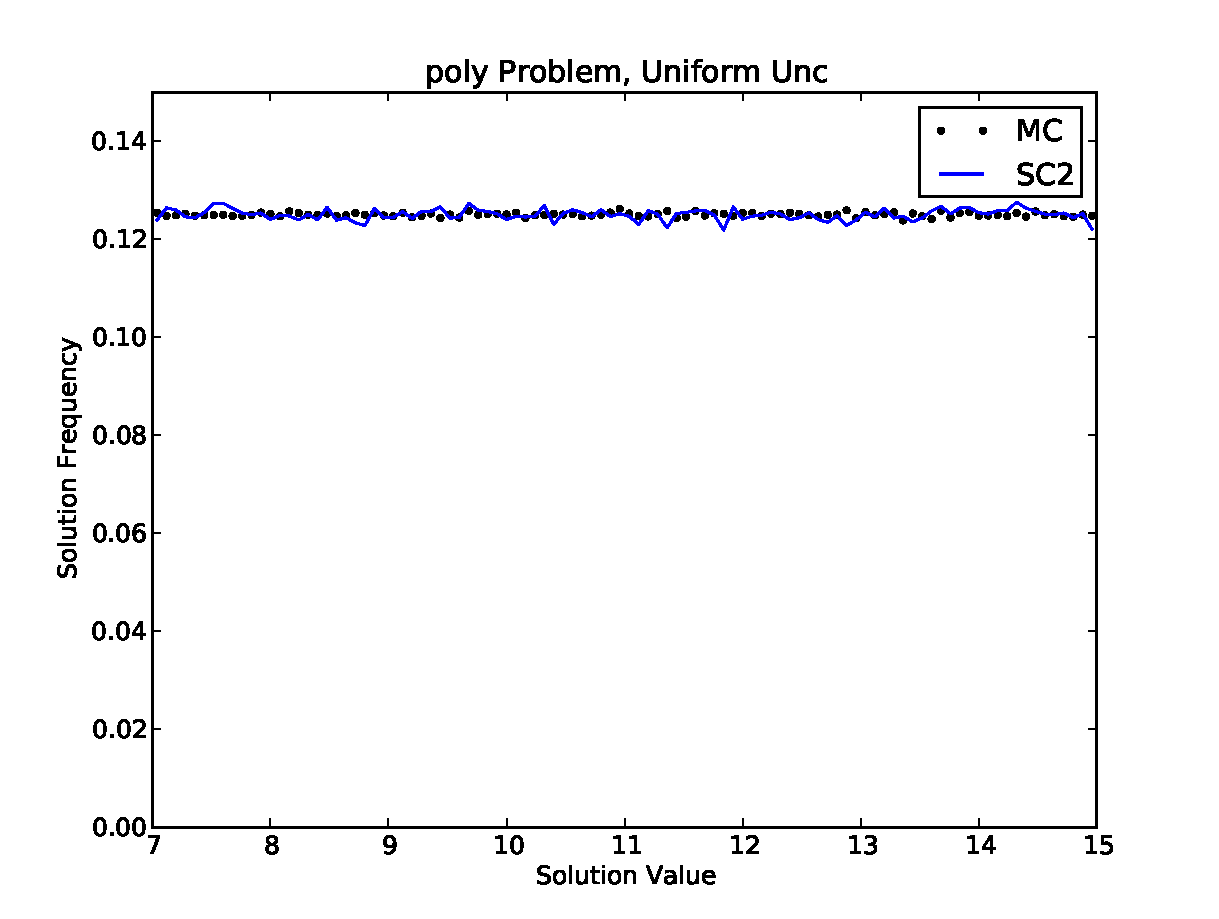
\includegraphics[width=0.7\textwidth]{../graphics/poly_uniform_pdfs}
   \caption{Polynomial Problem, Uniform PDFs}
      \label{fig:poly uni}
%  \end{subfigure}
\end{figure}
\begin{figure}[h]
\centering
%  \begin{subfigure}[b]{0.45\textwidth}
   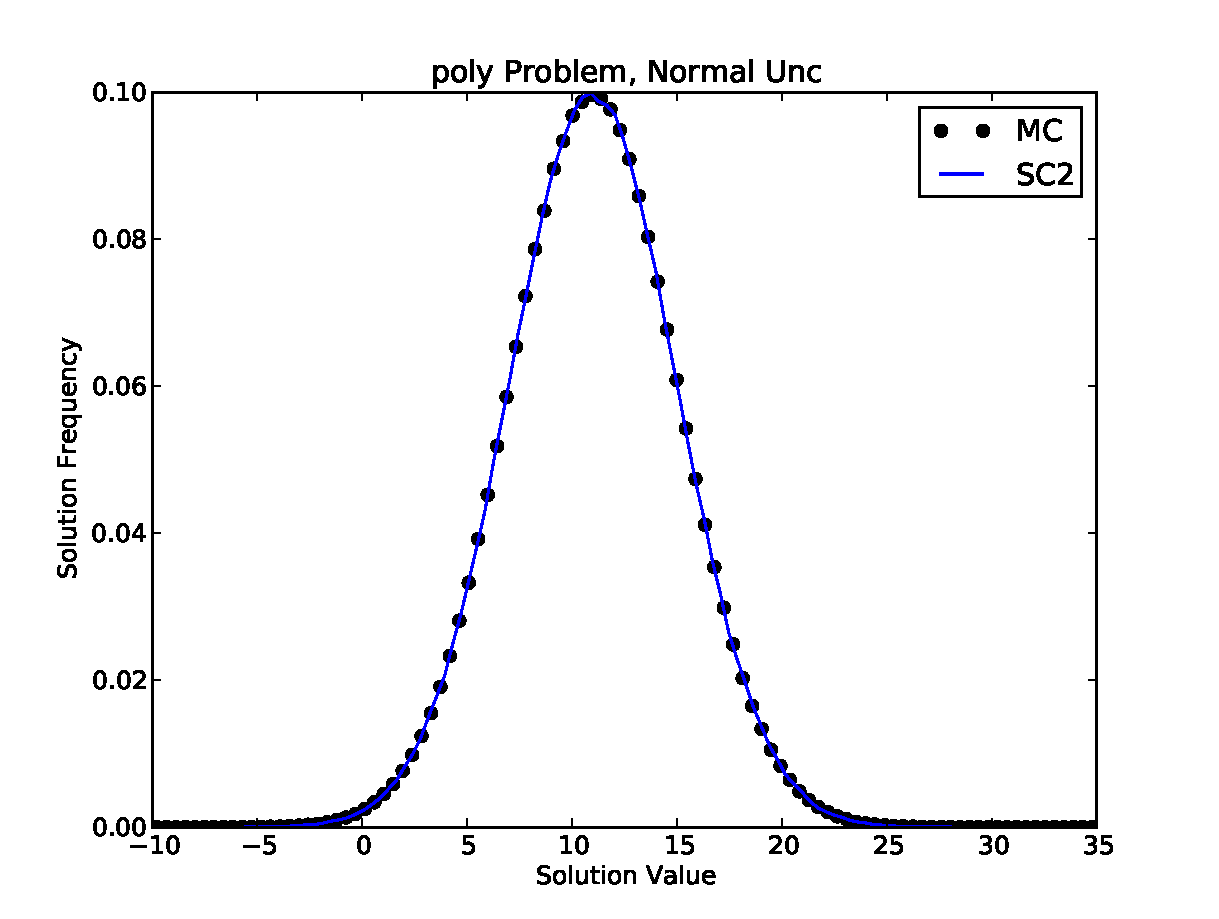
\includegraphics[width=0.7\textwidth]{../graphics/poly_normal_pdfs}
   \caption{Polynomial Problem, Normal PDFs}
      \label{fig:poly norm}
%  \end{subfigure}
%\caption{Polynomial Problem Solution Distributions}
%\label{fig:polypdfs}
\end{figure}



\subsection{Bivariate}
Similar to the univariate case, we add a dimension and define a new function to sample
\begin{equation}
U(\vb*{\theta})=U(\theta_1,\theta_2)=\theta_1\qty(1+\theta_2).
\end{equation}
We impose independence between the uncertain variables in $\vb*{\theta}$.
The expected value is given as
\begin{align}
\ev{U}&=\ev{\theta_1}+\ev{\theta_1\theta_2},\\
  &= \ev{\theta_1}\qty(1+\ev{\theta_2}).
\end{align}
The second moment is
\begin{align}
\ev{U^2}=\ev{\theta_1^2}\qty(1+2\ev{\theta_2}+\ev{\theta_2^2}).
\end{align}

\subsubsection{Uniform}
We allow $\vb*{\theta}$ to vary uniformly as
\begin{align}
\theta_1 &\in[3,7],\\
\theta_2 &\in[1,6].
\end{align}
Using the derivations for the univariate uniform variable, moments are given explicitly by
\begin{align}
\ev{U}&=(5)+(5)\qty(\frac{7}{2}), \\
  &= \frac{45}{2}.\\
\ev{U^2} &= \frac{(3)^2+(3)(7)+(7)^2}{3}\qty(1+(1+6)+\frac{(1)^2+(1)(6)+(6)^2}{3}),\\
  &= 588.\bar1.
\end{align}
The variance is
\begin{equation}
\text{var}[U]=\ev{U^2}-\ev{U}^2=79.08\bar3.
\end{equation}
%\section{Semi-Infinite Uniform Source}
This case is also an evaluation of an analytic function, but can't be exactly represented by a finite polynomial expansion.  The solution models the mono-energetic neutron flux at a point inside a 1D semi-infinite homogenous absorbing medium with a uniform source.  The governing PDE for this equation is
\begin{equation}
-D\ddrv{\phi}{x}+\Sigma_a\phi = S,
\end{equation}
and its solution is
\begin{equation}
\phi(S,D,x,\Sigma_a)=\frac{S}{\Sigma_a}\left(1-e^{-x/L}\right),
\end{equation}
\begin{equation}
L^2\equiv \frac{D}{\Sigma_a}.
\end{equation}
where $S$ is the uniform source, $\Sigma_a$ is the material's macroscopic absorption cross section, $D$ is the material's diffusion coefficient, $x$ is a distance into the medium from the boundary, and $\phi$ is the neutron flux.  Restated in the form used by PCESC,
\begin{equation}
U(p;\theta) = \frac{S}{\theta}\left(1-e^{-\sqrt{\theta} x/\sqrt{D}}\right),
\end{equation}
where $p=(S,D,x)$.  
We consider the cases when the absorption cross section $\theta$ has a uniform distribution as well as a normal distribution.   For both cases, parameters $p$ are as follows.
\begin{align}
S &= 1.0 \text{ n/cm}^2\text{/s},\\
D &= 0.5 \text{ /cm},\\
x &= 2.0 \text{ cm}.
\end{align}

We allow $\Sigma_a$ to vary uniformly as $\Sigma_a\in[0.5,1]$ or normally as $\Sigma_a\in\mathcal{N}(0.75,0.15)$ and quantify the uncertainty using PCESC as well as Monte Carlo sampling.
For increasing orders of expansion, the mean and variance obtained are shown along with the run time and are shown in Tables \ref{tab:source uni} and \ref{tab:source norm}.
\begin{table}
\begin{center}
\begin{tabular}{c c|l l}
type & runs/order & mean & variance \\ \hline
MC & $1\times10^6$ & 1.26069628111 & 0.0632432419713\\
SC & 2 & 1.25774207229 & 0.0495341371244 \\
SC & 4 & 1.26064320417 & 0.0604388749588 \\
SC & 8 & 1.26108375978 & 0.0637370898233\\
SC & 16 & 1.26112339681 & 0.0639754882641
\end{tabular}
\end{center}
\caption{Statistics for Source Problem with Uniform Uncertainty}
\label{tab:source uni}
\end{table}

\begin{table}[h!]
\begin{center}
\begin{tabular}{c c|l l| r}
type & runs/order & mean & variance & run time (sec) \\ \hline
MC & 23400 & 1.24922240195 & 0.0488719424418 & 366.31\\
SC & 2 & 1.2547221522 & 0 & 2.08 \\
SC & 4 & 1.25569029702 & 0.049198975952 & 3.11 \\
SC & 8 & 1.25569096924 & 0.0492316191443 & 4.74\\
SC & 16 & 1.25569096924 & 0.0492316191611 & 6.88
\end{tabular}
\end{center}
\caption{Statistics for Source Problem with Normal Uncertainty}
\label{tab:source norm}
\end{table}

\begin{figure}[h]
\centering
  \begin{subfigure}[b]{0.45 \textwidth}
   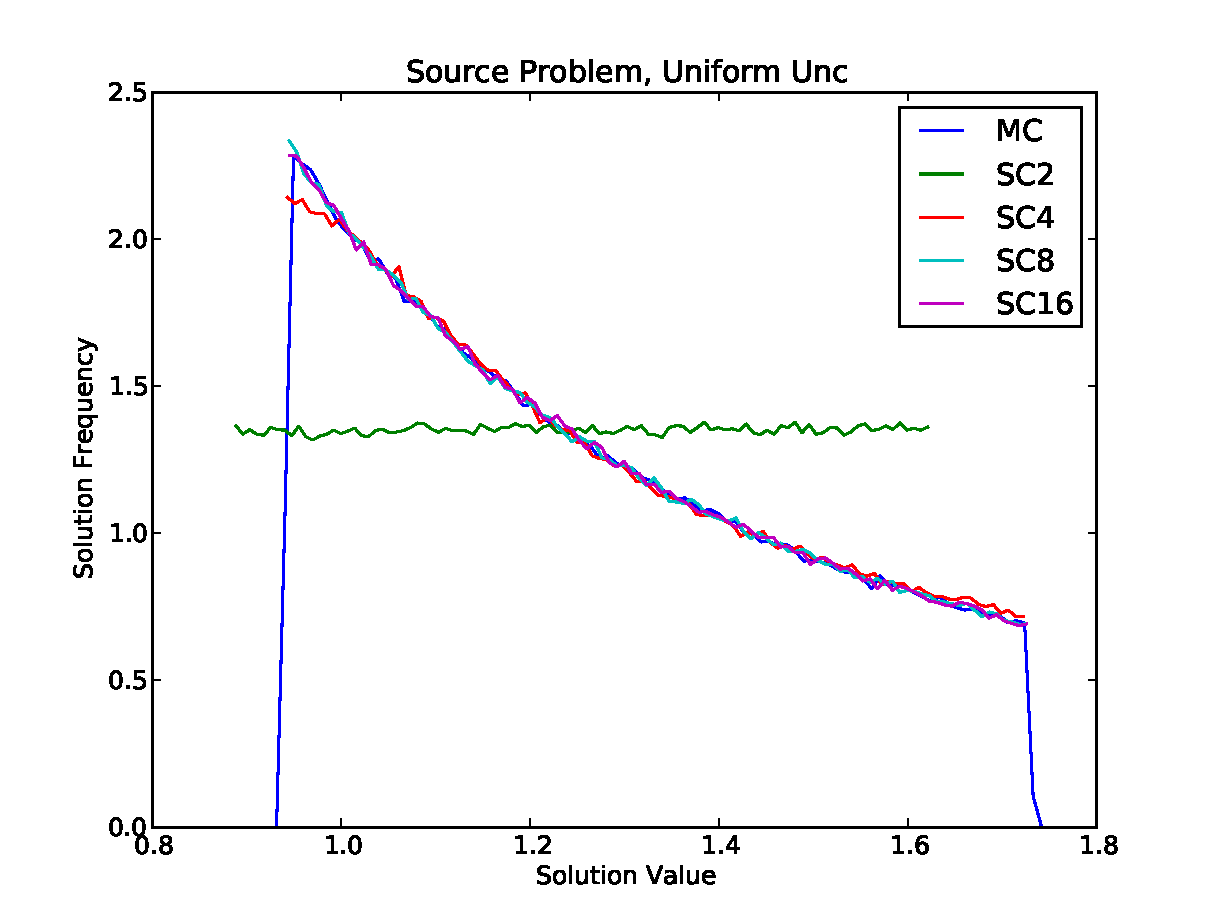
\includegraphics[width=\textwidth]{../graphics/source_uniform_pdfs}
   \caption{Uniform PDFs}
      \label{uni}
  \end{subfigure}
  \begin{subfigure}[b]{0.45\textwidth}
   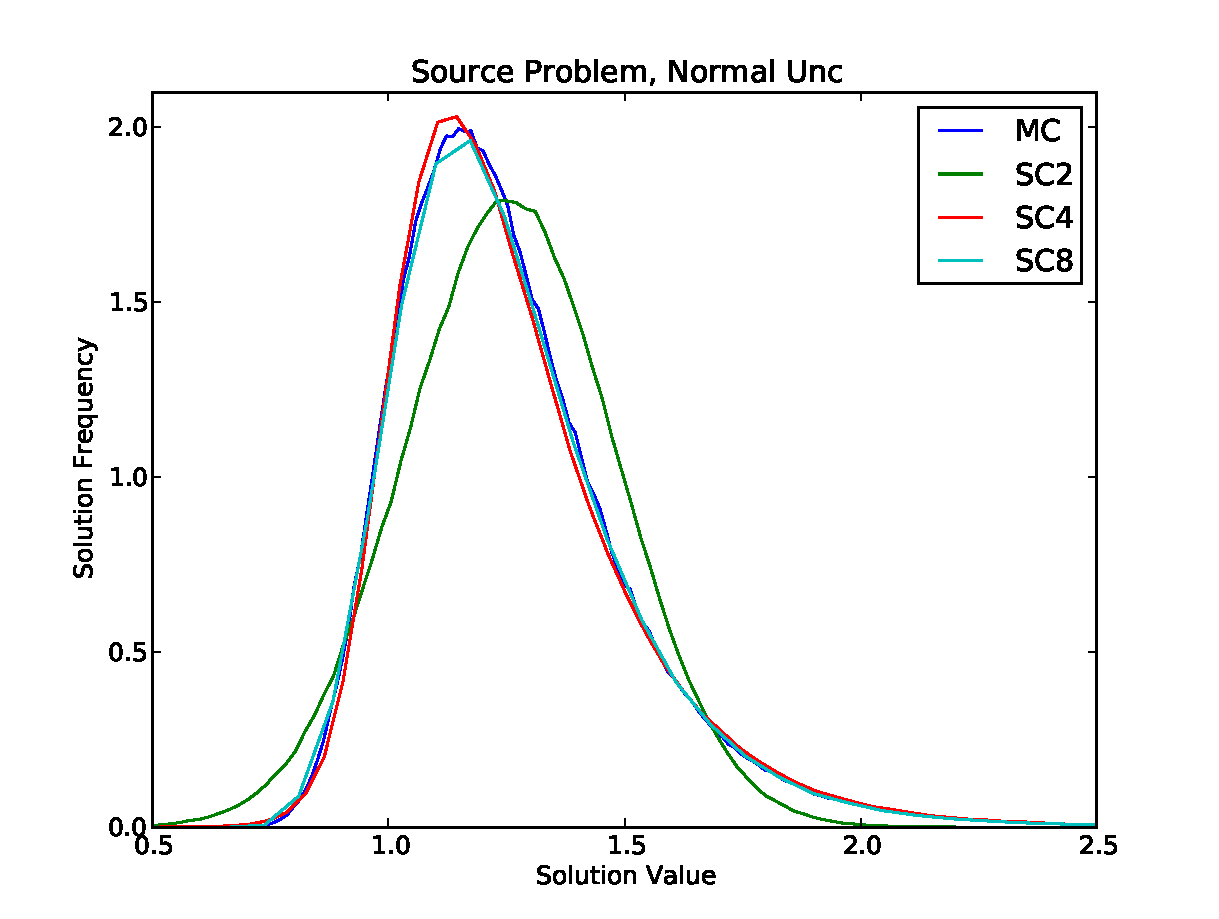
\includegraphics[width=\textwidth]{../graphics/source_normal_pdfs}
   \caption{Normal PDFs}
      \label{norm}
  \end{subfigure}
\caption{Source Problem Solution Distributions}
\label{fig:sourcepdfs}
\end{figure}

The PDFs were obtained by Monte Carlo sampling of the ROM for the PCESC cases, and obtained directly for the Monte Carlo case, shown in Fig. \ref{fig:sourcepdfs}.  The x-axis is the value of the scalar flux, and the y-axis is the probability of obtaining a particular flux.


%\begin{table}
%\begin{center}
%\begin{tabular}{c c|l l| r}
%type & runs/order & mean & variance & run time (sec) \\ \hline
%MC & 1\times10^6 &  &  & \\
%SC & 2 & & & \\
%SC & 4 & & & \\
%SC & 8 & & & \\
%SC & 16 & & &
%\end{tabular}
%\end{center}
%\caption{}
%\label{}
%\end{table}
%
%\begin{figure}[h!]
%\centering
%   \includegraphics[width=\textwidth]{../graphics/}
%   \label{}
%   \caption{}
%\end{figure}

%\section{1D 2G Homogeneous}
This problem is a simple version of a $k$-eigenvalue criticality problem using neutron diffusion.  While this problem is 1D, we use a 2D mesh to solve it by imposing reflecting boundary conditions on the top and bottom.  The governing PDE for this equation is
\begin{equation}
-\drv{}{x}D_g\drv{\phi_g}{x}+(\Sigma_{g,a}+\Sigma_{g,s})\phi_g = \sum_{g'}\sigma_{s}^{g'\to g}\phi_{g'} + \frac{\chi_{g}}{k}\sum_{g'}\nu_{g'}\sigma_{f,g'}\phi_{g'},\hspace{15pt} g\in[1,2],
\end{equation}
\begin{equation}
\Sigma_{g,a}=\Sigma_{g,\gamma}+\Sigma_{g,f},
\end{equation}
where $g$ denotes the energy group, $D$ is the group diffusion cross section; $\phi$ is the group flux, $x$ is the location within the problem; $\Sigma_a,\Sigma_s,\Sigma_f,\Sigma_\gamma$ are the macroscopic absorption, scattering, fission, and capture cross sections respectively; $k$ is the criticality factor eigenvalue and quantity of interest; and $\chi$ is the fraction of neutrons born into an energy group.  In this case, we consider only downscattering, and fission neutrons are only born into the high energy group ($\Sigma_s^{2\to1}=\chi_2=0$).

This problem does not have a convenient general analytic solution.  We can express the solver as
\begin{equation}
U(p;\theta) = k(p;\Sigma_{2,\gamma}),
\end{equation}
where
\begin{equation}
p=(D_g,\Sigma_{1,\gamma},\Sigma_{g,s},\nu_g,\Sigma_{g,f},\chi_g),\hspace{20pt}g\in[1,2].
\end{equation}
While $\phi_g(x)$ might also be considered a parameter, it is an output value solved simultaneously with $k$.

For this test code we consider $\theta=\Sigma_{2,\gamma}$ in three possible normal distributions.  Evaluated at the distribution mean of $\theta$, we consider one each case where $k=(0.9,1.0,1.1)$, given by the distributions $\theta\in\mathcal{N}(0.055969,0.1), \theta\in\mathcal{N}(0.04438,0.1), \theta\in\mathcal{N}(0.035181,0.1)$ respectively.  

It is important to note that the Monte Carlo sampling was restricted to values within 3 standard deviations of the mean; as such, the means and variances obtained directly through Monte Carlo sampling are not representative of the full uncertainty space.  This truncation of the distribution is enforced because without such a restriction, it is possible to sample physically untenable values for $\Sigma_{2,a}$, including negative values.

A summary of all three cases is shown in Fig. \ref{1d_all}.  Tabular data for mean and variance convergence is in Tables \ref{tab:1dcrit} to \ref{tab:1dsub}, where the clock time shown makes use of embarrassingly-parallel Monte Carlo sampling with 4 cores.  The times for the PCESC runs include the construction of the ROM prior to sampling.  The pdfs for each case are in Figs. \ref{fig:1d 3pdfs}.  

\begin{figure}[h!]
\centering
   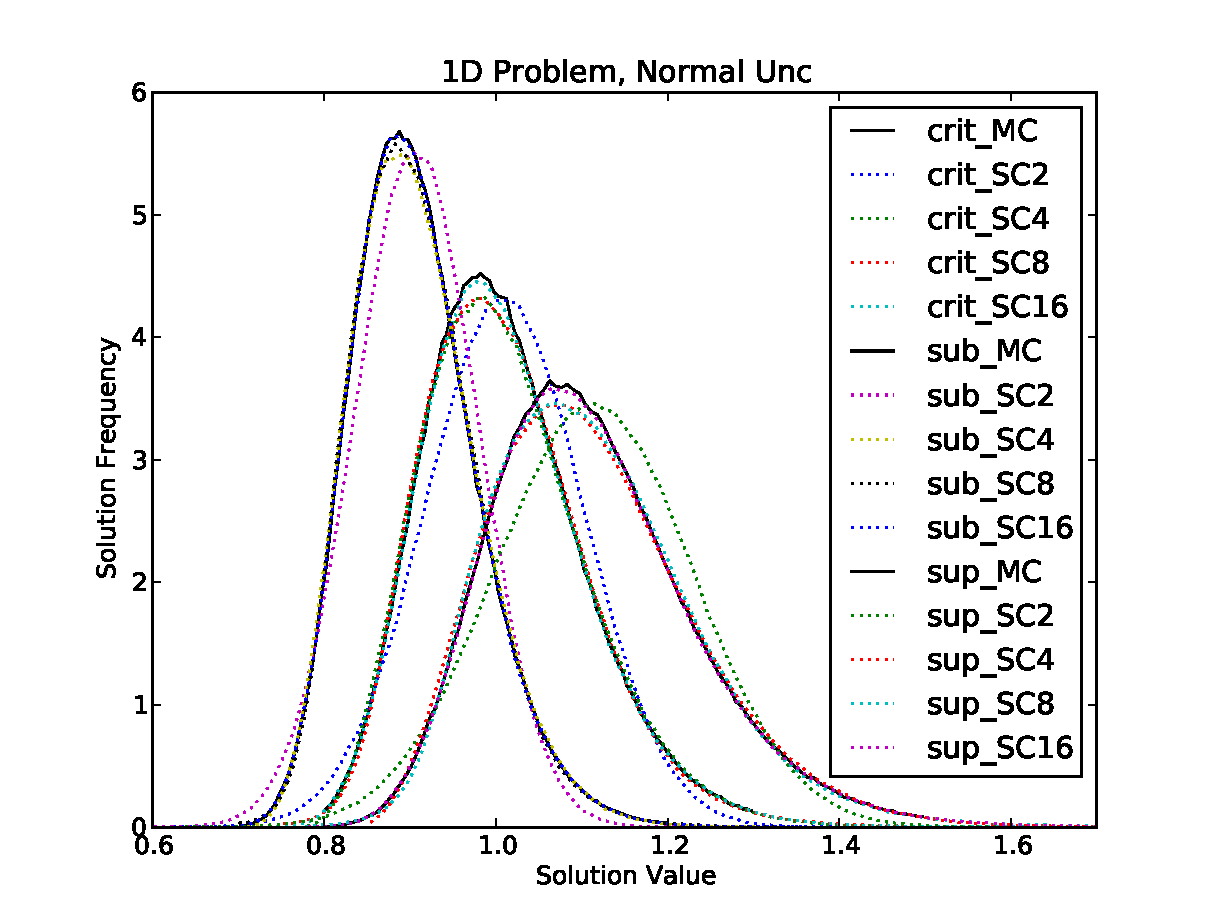
\includegraphics[width=.75\textwidth]{../graphics/1dall_normal_pdfs}
   \caption{Summary, 1D Criticality}
   \label{1d_all}
\end{figure}

\begin{table}
\begin{center}
\begin{tabular}{c c|l l l}
type & runs/order & mean & variance & time (s) \\ \hline
MC & $1\times10^6$ & 1.01144778738 & 0.0105716289269 & 15082  \\
SC & 2 & 1.01107577584 & 0.00974910361412 & 133 \\
SC & 4 & 1.0113755955 & 0.0105739848126 & 231\\
SC & 8 & 1.01137628238 & 0.0105785232446 & 450\\
SC & 16 & 1.01137628243 & 0.0105785241745 & 862
\end{tabular}
\end{center}
\caption{Convergence of Mean, Variance for Critical Case}
\label{tab:1dcrit}
\end{table}

\begin{table}
\begin{center}
\begin{tabular}{c c|l l}
type & runs/order & mean & variance \\ \hline
MC & $1\times10^6$ & 1.11593980088 & 0.0168503796482 \\
SC & 2 & 1.11537873568 & 0.0151539223359 \\
SC & 4 & 1.11590698755 & 0.016795821961\\
SC & 8 & 1.11590896034 & 0.0168106966474 \\
SC & 16 & 1.11590896088 & 0.0168107061554
\end{tabular}
\end{center}
\caption{Convergence of Mean, Variance for Supercritical Case}
\label{tab:1dsup}
\end{table}

\begin{table}
\begin{center}
\begin{tabular}{c c|l l}
type & runs/order & mean & variance \\ \hline
MC & $1\times10^6$ & 0.907699673282 & 0.00632790358771 \\
SC & 2 & 0.907653521565 & 0.00595095987773 \\
SC & 4 & 0.907813174929 & 0.00633526057266\\
SC & 8 & 0.907813389468 & 0.00633649118503 \\
SC & 16 & 0.907813389471 & 0.00633649126226
\end{tabular}
\end{center}
\caption{Convergence of Mean, Variance for Subcritical Case}
\label{tab:1dsub}
\end{table}

\subsection{Chaos Moment Quadrature Convergence}
One concern with using stochastic collocation to build the polynomial chaos moments is the appropriate order of quadrature to use.  With Gaussian quadrature, a sum with $n$ terms can exactly integrate a polynomial of order $2n-1$.  The chaos moment expression we integrate is
\begin{align}
c_i &= \int_\Omega U(\theta)P(\theta)B_i(\theta)d\theta,\\
  &\approx \sum_{\ell=0}^L w_\ell U(\theta_\ell)B_i(\theta_\ell),
\end{align}
where $P$ is the probability distribution of $\theta$ and $B_i$ is the $i-th$ order basis polynomial.  In the simplest case when $U(\theta)$ is a scalar quantity, the order of the expression under the integral is determined solely by the basis polynomial.  Thus a quadrature order of $(i+1)/2$ is the minimum quadrature order necessary to integrate the chaos moments.  In the case $U(\theta$) is highly nonlinear and ill-approximated by even high-order polynomials, the necessary quadrature order required to accurately determine moments could be much higher.

As an example of chaos moment convergence as a function of quadrature order, we show the PCESC moments of the critical case for 8th-order quadrature in Table \ref{tab:quadconverge}, as determined by increasing orders of quadrature from the minimum to 12-th order, which assumes $U(\theta)$ is well-approximated by a 7th-order polynomial.  As can be seen, the lower moments require smaller quadrature orders, and at least order 8 quadrature is necessary to see reasonable convergence for higher moments.  In addition, the moments calculated using quadrature order equal to expansion order are given for expansion orders 2 to 32 in Fig. \ref{tab:1dcrit coeffs}.
\begin{landscape}
\begin{table}[H]
\begin{center}
\begin{tabular}{c | *{8}{l}}
Order & 1 & 2 & 3 & 4 & 5 & 6 & 7 & 8 \\ \hline
5 & 1.34648094 & -0.13502447 & 0.02226791 & -0.0045477 & 0.00000000 & 0.00101863 & -0.00092988 & 0.00313821\\
6 & 1.34648100 & -0.13502501 & 0.02227125 & -0.00456451 & 0.0010908 & -0.00027317 &  0.00000000 & 0.00025291\\ 
8 & 1.34648101 & -0.13502506 & 0.02227158 & -0.00456614 & 0.0010978 & -0.00029964 & 9.01120742e-05 & -2.67010906e-05\\ 
10& 1.34648101 & -0.13502506 & 0.02227158 & -0.00456616 & 0.0010979 & -0.00030000 & 9.13419949e-05 & -3.05173759e-05\\ 
12& 1.34648101 & -0.13502506 & 0.02227158 & -0.00456616 & 0.0010979 & -0.00030001 & 9.13732306e-05 & -3.06142832e-05
\end{tabular}
\end{center}
\caption{Chaos Moment Convergence with Increasing Quadrature Order}
\label{tab:quadconverge}
\end{table}
\vspace{50pt}
\begin{figure}[H]
\centering
\begin{subfigure}[b]{0.43\textwidth}
   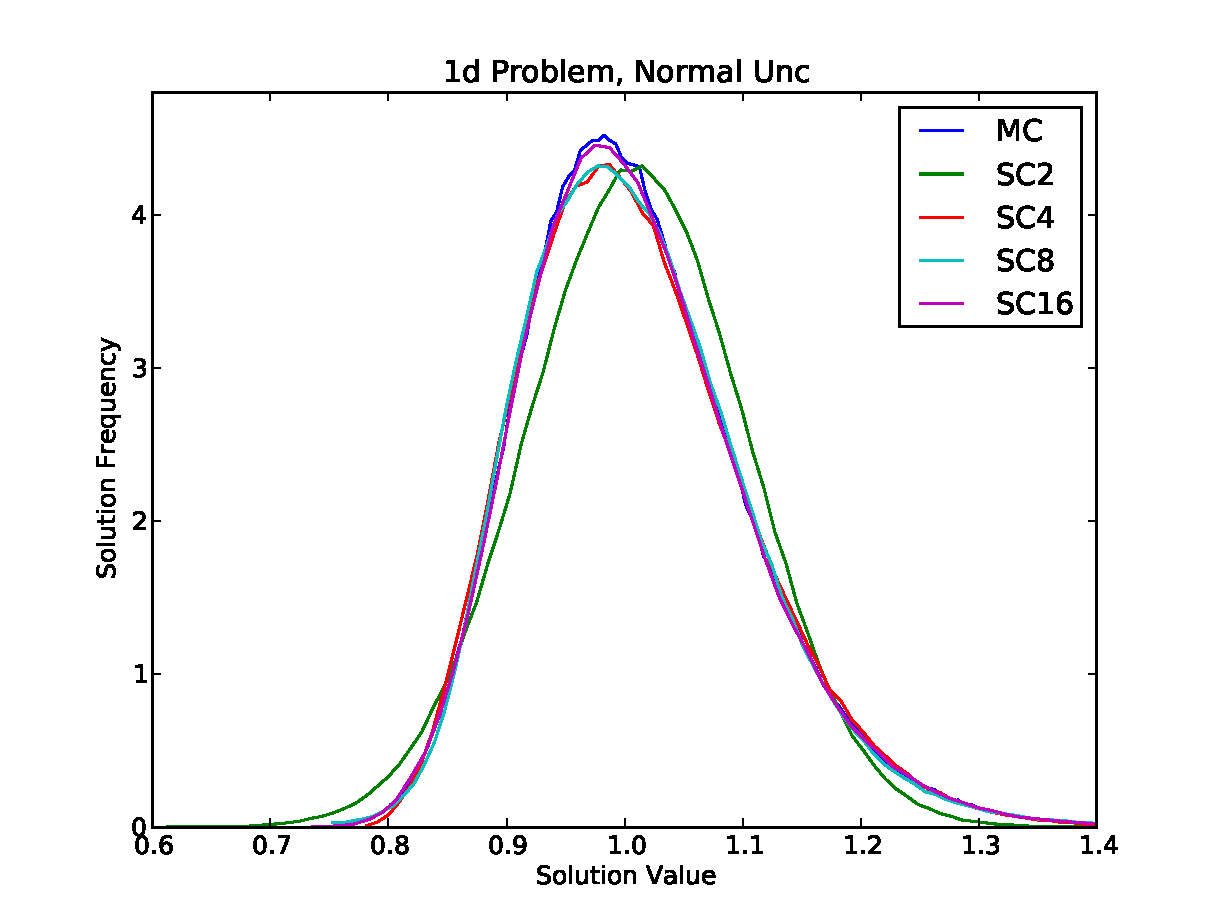
\includegraphics[width=\textwidth]{../graphics/1d_normal_pdfs}
   \caption{Critical}
   \label{fig:1dcrit}
\end{subfigure}
\begin{subfigure}[b]{0.43\textwidth}
   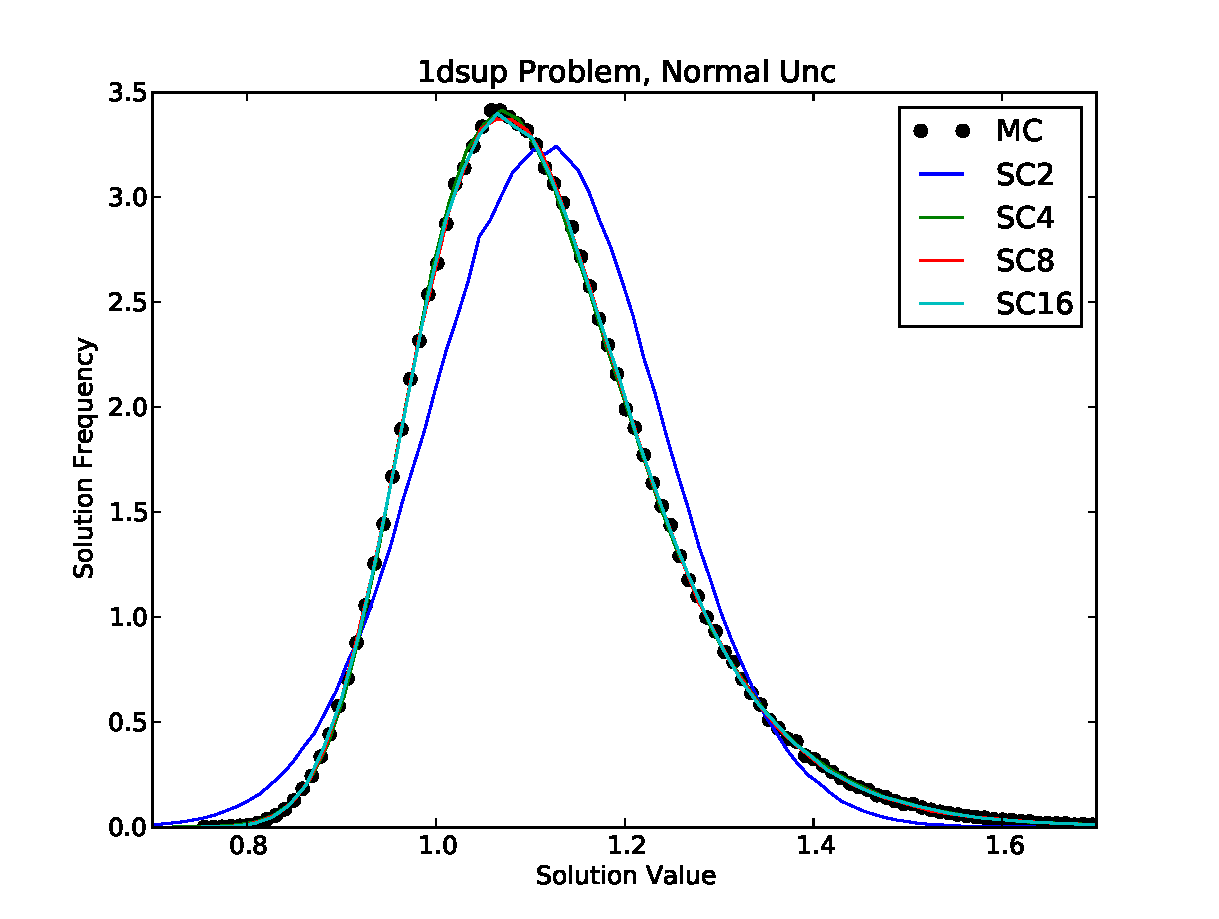
\includegraphics[width=\textwidth]{../graphics/1dsup_normal_pdfs}
   \caption{Supercritical}
      \label{fig:1dsup}
\end{subfigure}
\begin{subfigure}[b]{0.43\textwidth}
   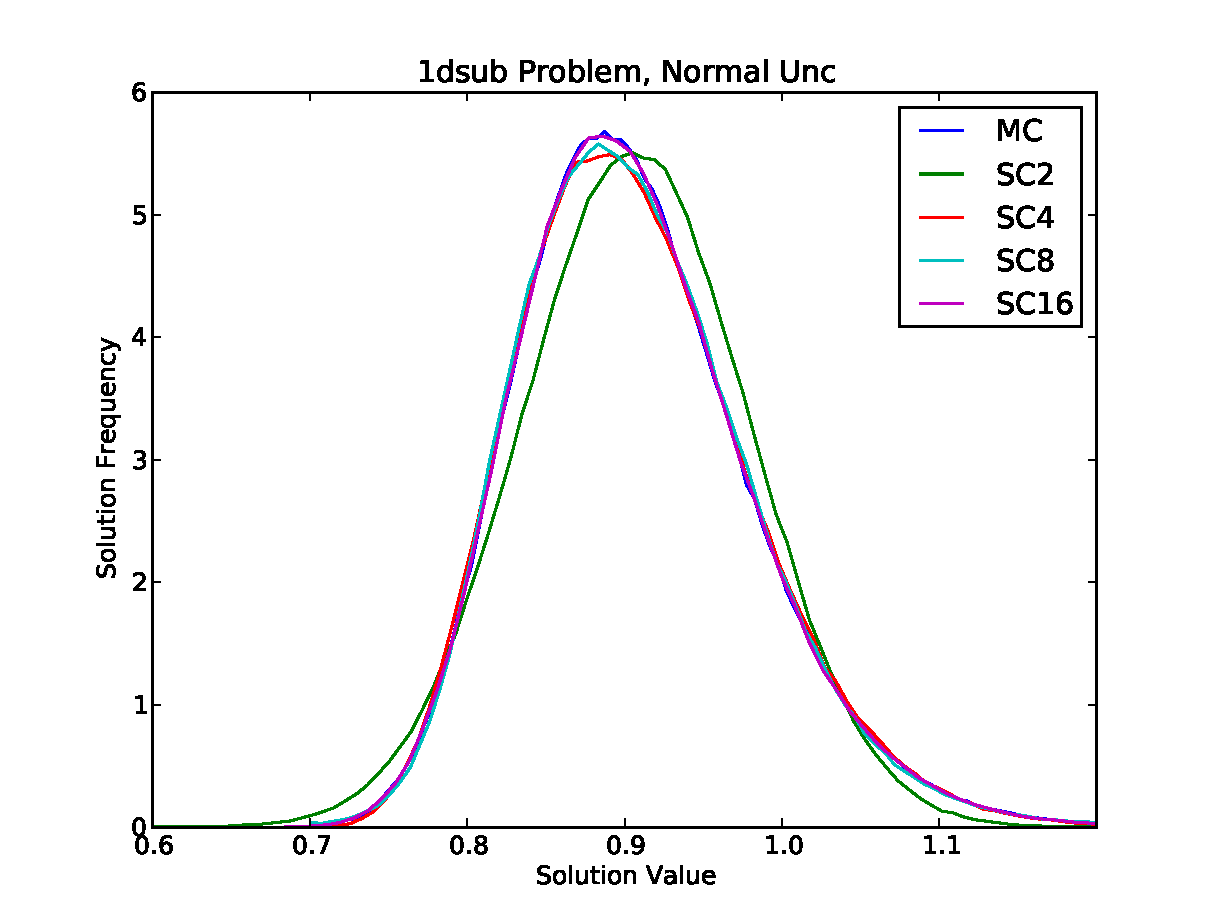
\includegraphics[width=\textwidth]{../graphics/1dsub_normal_pdfs}
   \caption{Subcritical}
      \label{fig:1dsub}
\end{subfigure}
\caption{1D Solution PDF Convergences}
\label{fig:1d 3pdfs}
\end{figure}
\end{landscape}

\begin{table}[H]
\begin{center}
\begin{tabular}{c | l l l l l}
Moment & SC2 & SC4 & SC8 & SC16 & SC32\\ \hline
1 & 1.34608094 & 1.3464801 & 1.34648101 & 1.34648101 &  1.34648101\\
2 & -0.13145279 & -0.1350169 & -0.13502506 & -0.13502506 &  -0.13502506\\ 
3 & 0 & 0.02222067 & 0.02227158 & 0.02227158 &  0.02227158\\ 
4 & 0 & -0.00431037 & -0.00456614 & -0.00456616 & -0.00456616 \\ 
5 & 0 & 0 & 0.0010978 & 0.0010979 & 0.0010979 \\ 
6 & 0 & 0 & -0.00029964 & -0.00030001 & -0.00030001 \\ 
7 & 0 & 0 & 9.01120742e-05 & 9.13747084e-05 & 9.13746830e-05 \\ 
8 & 0 & 0 & -2.67010906e-05 & -3.06188612e-05 & -3.06187650e-05 \\ 
9 & 0 & 0 & 0 & 1.11868181e-05 & 1.11865704e-05 \\ 
10 & 0 & 0 & 0 & -4.42800671e-06 & -4.42735312e-06 \\ 
11 & 0 & 0 & 0 & 1.89021407e-06 & 1.88853134e-06 \\ 
12 & 0 & 0 & 0 & -8.66874281e-07 & -8.62852707e-07 \\ 
13 & 0 & 0 & 0 & 4.24658199e-07 & 4.15693998e-07 \\ 
14 & 0 & 0 & 0 & -2.18790217e-07 & -1.99976426e-07 \\ 
15 & 0 & 0 & 0 & 1.12938059e-07 & 7.56801496e-08 \\ 
16 & 0 & 0 & 0 & -4.90000878e-08 & 2.05894301e-08 \\ 
17 & 0 & 0 & 0 & 0 & -1.22580841e-07 \\ 
18 & 0 & 0 & 0 & 0 & 2.51097599e-07 \\ 
19 & 0 & 0 & 0 & 0 & -4.18278488e-07 \\ 
20 & 0 & 0 & 0 & 0 & 6.25910592e-07 \\ 
21 & 0 & 0 & 0 & 0 & -8.61060458e-07 \\ 
22 & 0 & 0 & 0 & 0 & 1.09209939e-06 \\ 
23 & 0 & 0 & 0 & 0 & -1.26866179e-06 \\ 
24 & 0 & 0 & 0 & 0 & 1.32892404e-06 \\ 
25 & 0 & 0 & 0 & 0 & -1.21597330e-06 \\ 
26 & 0 & 0 & 0 & 0 & 9.01437926e-07 \\ 
27 & 0 & 0 & 0 & 0 & -4.09433059e-07 \\ 
28 & 0 & 0 & 0 & 0 & -1.70599526e-07 \\ 
29 & 0 & 0 & 0 & 0 & 6.94034499e-07 \\ 
30 & 0 & 0 & 0 & 0 & -9.99892578e-07 \\ 
31 & 0 & 0 & 0 & 0 & 9.71463606e-07 \\ 
32 & 0 & 0 & 0 & 0 & -5.97051529e-07 \\ 
\end{tabular}
\end{center}
\caption{Chaos Moments for 1D Critical Case}
\label{tab:1dcrit coeffs}
\end{table}
%
%\begin{figure}[h!]
%\centering
%   \includegraphics[width=\textwidth]{../graphics/}
%   \label{}
%   \caption{}
%\end{figure}
%\begin{table}
%\begin{center}
%\begin{tabular}{c c|l l| r}
%type & runs/order & mean & variance & run time (sec) \\ \hline
%MC & 1\times10^6 &  &  & \\
%SC & 2 & & & \\
%SC & 4 & & & \\
%SC & 8 & & & \\
%SC & 16 & & &
%\end{tabular}
%\end{center}
%\caption{}
%\label{}
%\end{table}
%
%\begin{figure}[h!]
%\centering
%   \includegraphics[width=\textwidth]{../graphics/}
%   \label{}
%   \caption{}
%\end{figure}

%\section{2D 2G Quarter Core}
\subsection{Equations}
This problem is a more traditional $k$-eigenvalue criticality problem using neutron diffusion.  We simulate a benchmark reactor core by imposing reflecting conditions on the left and bottom boundaries of a quarter-core geometry.  The governing PDE for this equation is still
\begin{equation}
-\drv{}{x}D_g\drv{\phi_g}{x}+(\Sigma_{g,a}+\Sigma_{g,s})\phi_g = \sum_{g'}\sigma_{s}^{g'\to g}\phi_{g'} + \frac{\chi_{g}}{k}\sum_{g'}\nu_{g'}\sigma_{f,g'}\phi_{g'},\hspace{15pt} g\in[1,2],
\end{equation}
\begin{equation}
\Sigma_{g,a}=\Sigma_{g,c}+\Sigma_{g,f},
\end{equation}
where $g$ denotes the energy group, $D$ is the group diffusion cross section; $\phi$ is the group flux, $x$ is the location within the problem; $\Sigma_a,\Sigma_s,\Sigma_f$ are the macroscopic absorption, scattering, and fission cross sections respectively; $k$ is the criticality factor eigenvalue and quantity of interest; and $\chi$ is the fraction of neutrons born into an energy group.  In this case, we consider only downscattering, and fission neutrons are only born into the high energy group ($\Sigma_s^{2\to1}=\chi_2=0$).  Our coupled equations are
\begin{equation}
-\drv{}{x}D_1\drv{\phi_1}{x}+(\Sigma_{1,a}+\Sigma_s^{1\to2})\phi_1 = \frac{1}{k}\sum_{g'=1}^2\nu_{g'}\sigma_{f,g'}\phi_{g'},
\end{equation}
\begin{equation}
-\drv{}{x}D_2\drv{\phi_2}{x}+\Sigma_{2,a}\phi_2 = \sigma_{s}^{1'\to 2}\phi_1,
\end{equation}
\begin{equation}
\Sigma_{g,a}=\Sigma_{g,c}+\Sigma_{g,f}.
\end{equation}

\subsection{Materials and Geometry}
The two-dimensional core is shown in Fig. \ref{coremap} and the material properties are listed in Table \ref{tab:coremats}.
\begin{figure}[h]
\centering
   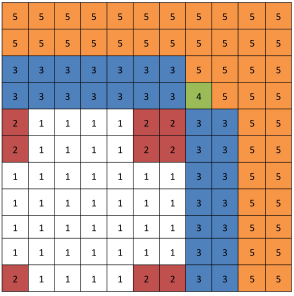
\includegraphics[width=0.4\textwidth]{../graphics/core}
   \caption{Core Map}
   \label{coremap}
\end{figure}
\begin{table}[h]
\centering
\begin{tabular}{c c | c c c c}
Region & Group & $D_g$ & $\Sigma_{c,g}$ & $\nu\Sigma_{f,g}$ & $\Sigma_s^{1,2}$ \\ \hline
1 & 1 & 1.255    & 4.602e-3 & 4.602e-3 & 2.533e-2 \\
  & 2 & 2.11e-1  & 5.540e-2 & 1.091e-1 & \\ \hline
2 & 1 & 1.268    & 4.609e-3 & 4.609e-3 & 2.767e-2 \\
  & 2 & 1.902e-1 & 8.675e-2 & 8.675e-2 & \\ \hline
3 & 1 & 1.259    & 6.083e-3 & 4.663e-3 & 2.617e-2 \\
  & 2 & 2.091e-1 & 4.142e-2 & 1.021e-1 & \\ \hline
4 & 1 & 1.259    & 4.663e-3 & 4.663e-3 & 2.617e-2 \\
  & 2 & 2.091e-1 & 3.131e-2 & 1.021e-1 & \\ \hline
5 & 1 & 1.257    & 6.034e-4  & 0 & 4.754e-2 \\
  & 2 & 1.592e-1 & 1.911e-2  & 0 & 
\end{tabular}
\caption{Basic Material Properties for Core}
\label{tab:coremats}
\end{table}

\subsection{Uncertainty Quantification}
This problem also does not have a convenient general analytic solution.  We can express the solver as
\begin{equation}
U(p;\theta) = k(p;\Sigma_{2,c}),
\end{equation}
where
\begin{equation}
p=(D_g,\Sigma_{1,c},\Sigma_{g,s},\nu_g,\Sigma_{g,f},\chi_g),\hspace{20pt}g\in[1,2].
\end{equation}
While $\phi_g(x)$ might also be considered a parameter, it is an output value solved simultaneously with $k$.

For this test code we consider $\theta=\Sigma_{2,c}$ normally distributed as $\theta\in\mathcal{N}(0.0554,0.01^2)$. Tabular data for mean and variance convergence is in Table \ref{tab:2dcrit}, and the pdfs obtained are in Fig. \ref{fig:2dcrit}.  Once again, it is important to note that the Monte Carlo sampling was restricted to values within 3 standard deviations of the mean; as such, the means and variances obtained directly through Monte Carlo sampling are not representative of the full uncertainty space.  This truncation of the distribution is enforced because without such a restriction, it is possible to sample physically untenable values for $\Sigma_{2,c}$, including negative values.

The PCESC runs all made use of order 32 quadrature to integrate chaos moments.

\begin{table}
\begin{center}
\begin{tabular}{c c|l l}
type & runs/order & mean & variance \\ \hline
MC & $6\times10^5$ & 1.01333702129 & 0.00160652595587 \\
SC & 2  & 1.01643813464 & 0.00138703446968 \\
SC & 4  & 1.01643813464 & 0.00184314998697 \\
SC & 8  & 1.01643813464 & 0.00184690058216 \\
SC & 16 & 1.01643813464 & 0.00184724103523 \\
SC & 32 & 1.01643813464 & 0.00184726152781
\end{tabular}
\end{center}
\caption{Convergence of Mean, Variance for 2D2G Case}
\label{tab:2dcrit}
\end{table}

\begin{figure}[h!]
\centering
   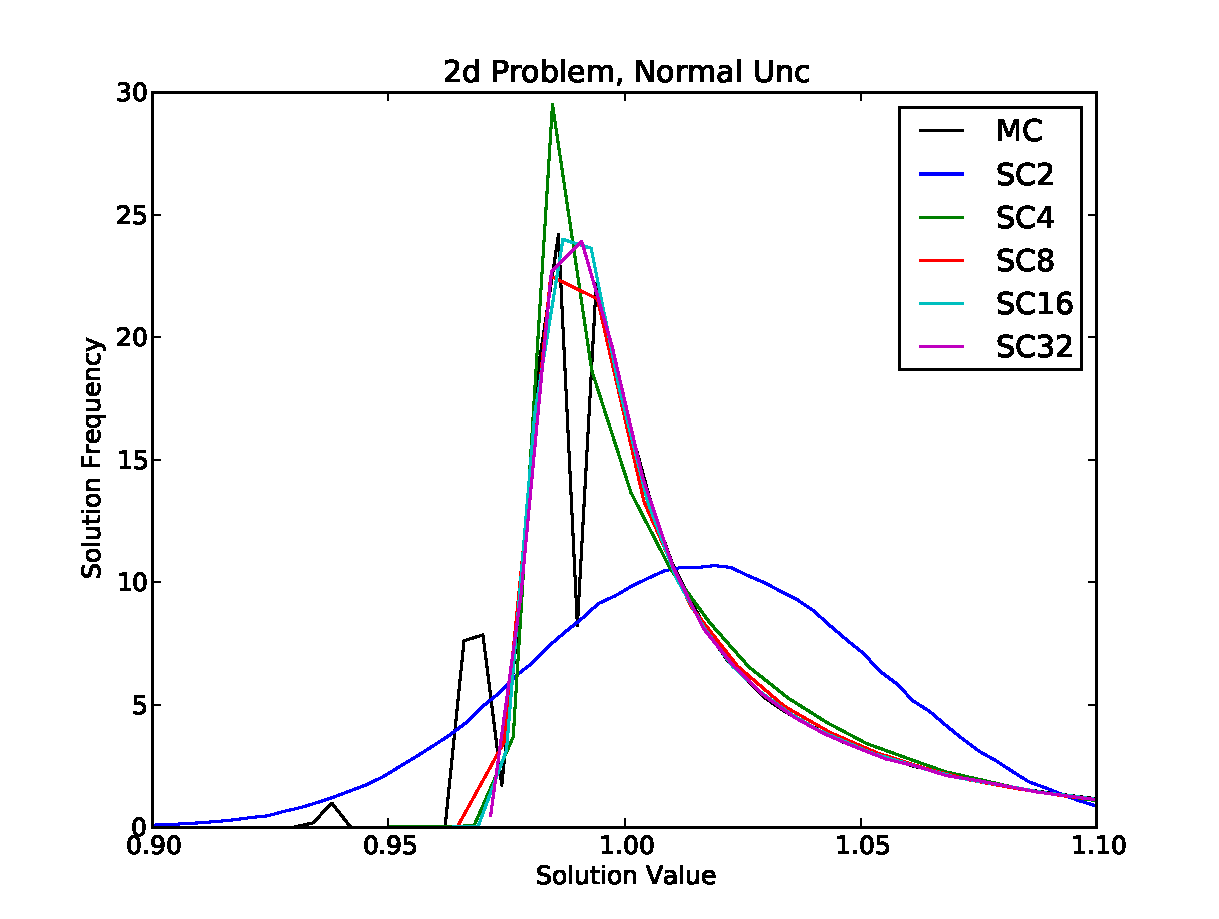
\includegraphics[width=\textwidth]{../graphics/2d_normal_pdfs}
   \caption{Solution PDF Convergence, 2D2G Case}
   \label{fig:2dcrit}
\end{figure}


%
%\begin{figure}[h!]
%\centering
%   \includegraphics[width=\textwidth]{../graphics/}
%   \label{}
%   \caption{}
%\end{figure}
%\begin{table}
%\begin{center}
%\begin{tabular}{c c|l l| r}
%type & runs/order & mean & variance & run time (sec) \\ \hline
%MC & 1\times10^6 &  &  & \\
%SC & 2 & & & \\
%SC & 4 & & & \\
%SC & 8 & & & \\
%SC & 16 & & &
%\end{tabular}
%\end{center}
%\caption{}
%\label{}
%\end{table}
%
%\begin{figure}[h!]
%\centering
%   \includegraphics[width=\textwidth]{../graphics/}
%   \label{}
%   \caption{}
%\end{figure}

\section{Conclusions}
In conclusion, we have shown that the PCESC uncertainty quantification algorithm shows good agreement with both analytic and Monte Carlo results for both univariate and multivariate uncertainty spaces.  The algorithm handles deterministic solvers in a ``black box'' sense, meaning it is agnostic of the complexity of the solver itself, as shown by four solvers ranging from simple polynomial evaluation to nonlinear multigroup diffusion.  In addition, we have shown that convergence for the PCESC method requires careful consideration of both quadrature order for each input parameter as well as the spatial discretization error of the deterministic solver.

We now turn our attention to the applicability of this algorithm.  Because of the exponential growth in expense for multivariate uncertainty spaces using the tensor product polynomial set, the efficiency of PCESC is lost when compared to Monte Carlo with the inclusion of many uncertain variables or a high degree polynomial expansion.  

There are, however, many more efficient methods for constructing the uncertainty space than using a full tensor product system.  We will explore sparse grid quadrature and analysis-of-variance style methods, as well as HDMR methods to reduce the necessary sample space and recovery the efficiency of the PCESC method.



\end{document}




\begin{center}
\begin{tabular}{c c|c c| c}
\end{tabular}
\end{center}

\begin{figure}[h]
\centering
  \begin{subfigure}[b]{0.45 \textwidth}
   \includegraphics[width=\textwidth]{}
   \caption{}
   \label{}
  \end{subfigure}
  \begin{subfigure}[b]{0.45\textwidth}
   \includegraphics[width=\textwidth]{}
   \caption{}
   \label{}
  \end{subfigure}
\caption{}
\end{figure}